\documentclass{article}
\usepackage{ctex}

\title{数字逻辑与计算机组成\\ {\small 实验 4: 加法器和 ALU 设计}}
\author{王卫东\quad 221900332}
\date{\zhtoday}

\usepackage{hyperref}
\usepackage{algorithm}
\usepackage{algorithmicx}
\usepackage{algpseudocode}
\usepackage{float}  
\usepackage{lipsum}
\usepackage{color, xcolor}
\usepackage{listings}
\usepackage{dirtree}
\usepackage{ulem}
\usepackage{graphicx}
\usepackage{amsmath}
\usepackage{amssymb}
\usepackage{amsfonts}
\usepackage{xcolor}
\usepackage{tikz}
\usepackage{multirow}
\usepackage{zhnumber} % change section number to chinese
\renewcommand\thesection{\zhnum{section}}
\renewcommand\thesubsection{\arabic{subsection}}
\usetikzlibrary{arrows,shapes,chains}

\begin{document}
    \maketitle

    \section{实验目的}

    \begin{enumerate}
        \item 掌握先行进位部件 CLU 和先行进位加法器 CLA 的设计方法。
        \item 掌握 32 位先行进位加法器的设计方法。
        \item 掌握 ALU 的设计方法。
    \end{enumerate}
    \section{实验环境}

    Logisim:https://github.com/Logisim-Ita/Logisim

    \section{实验内容}
    
    \subsection{4位先行进位部件CLU}

    \subsubsection{整体方案设计}
    \begin{figure}[H]
    \centering
    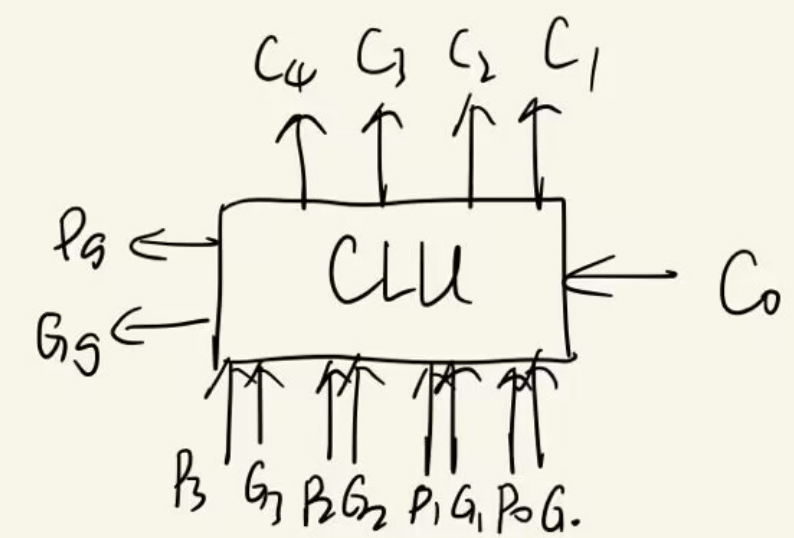
\includegraphics[width=0.4\textwidth]{1.1.png}
    \caption{4位先行进位部件CLU整体方案设计}
    \end{figure}

    \subsubsection{顶层模块设计}
    实验电路较为简单,不需要顶层模块设计图。

    \subsubsection{引脚作用}
    \begin{table}[H]
    \centering
    \begin{tabular}{|c|c|}
        \hline
        $C_{0}$  & 输入的最低位进位 \\ \hline
        $P_{0}\thicksim P_{3}$ & 输入的四位进位传递函数 \\ \hline
        $G_{0}\thicksim G_{3}$   & 输入的四位进位生成函数 \\ \hline
        $C_{0}\thicksim C_{3}$   & 向高位进位 \\ \hline
        $P_{g}$   & 输入的组间进位传递函数 \\ \hline
        $G_{g}$   & 输出的组间进位生成函数 \\ \hline
    \end{tabular}
    \caption{CLU引脚作用}
    \end{table}

    \subsubsection{原理图和电路图}
    \begin{figure}[H]
    \centering
    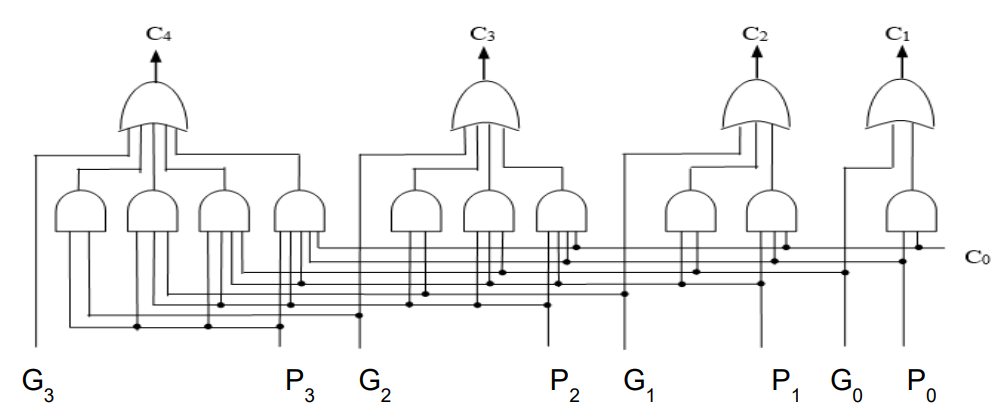
\includegraphics[width=0.8\textwidth]{1.4.1.png}
    \caption{CLU原理图}
    \end{figure}

    \begin{figure}[H]
    \centering
    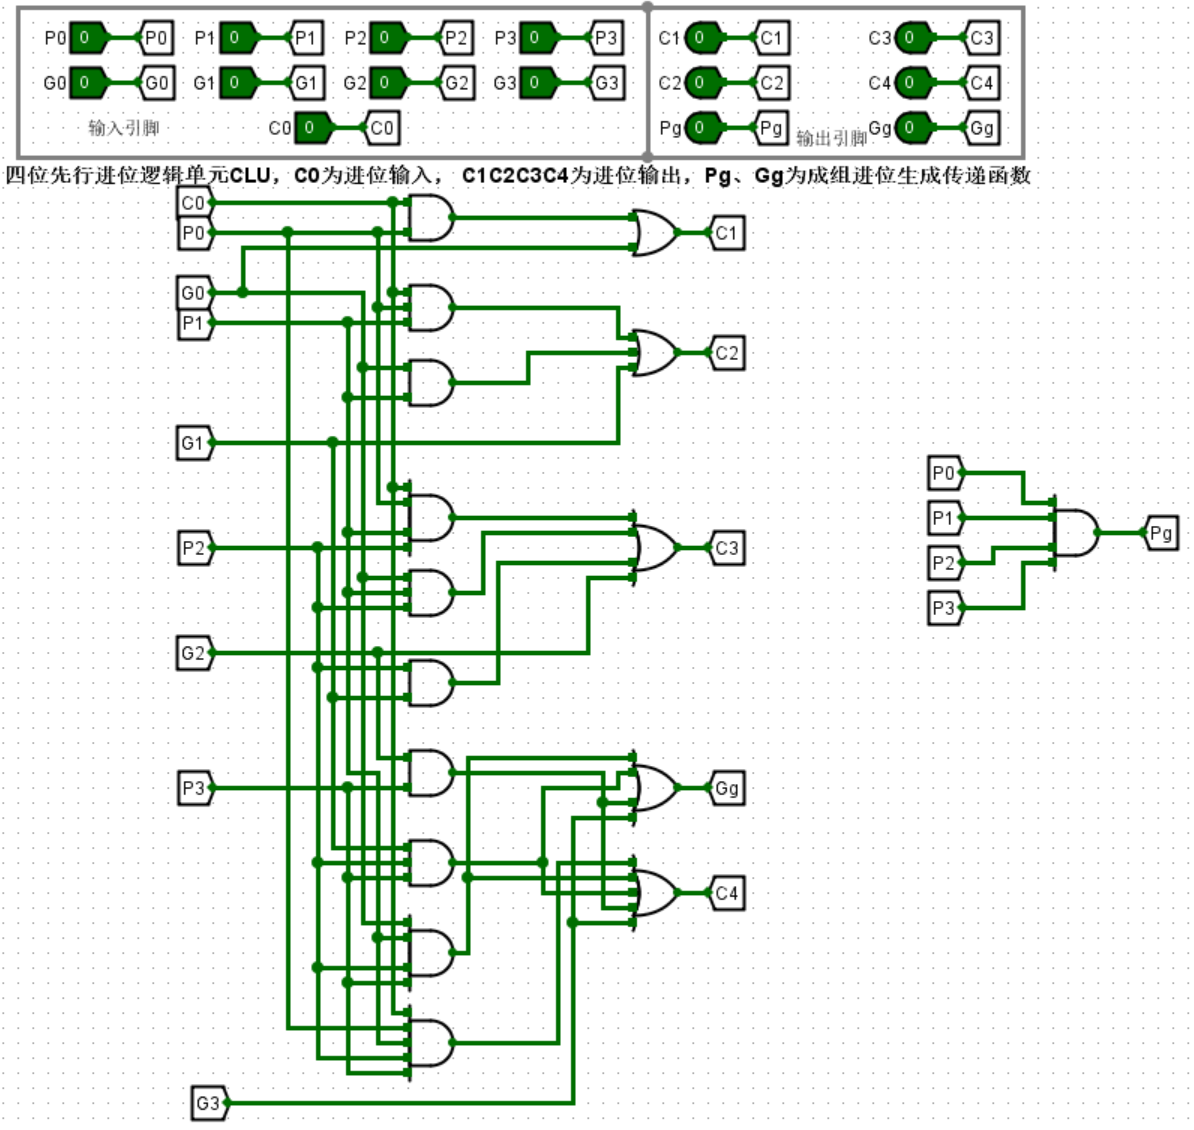
\includegraphics[width=0.8\textwidth]{1.4.2.png}
    \caption{CLU电路图}
    \end{figure}

    \subsubsection{仿真测试图}
    \begin{figure}[H]
    \centering
    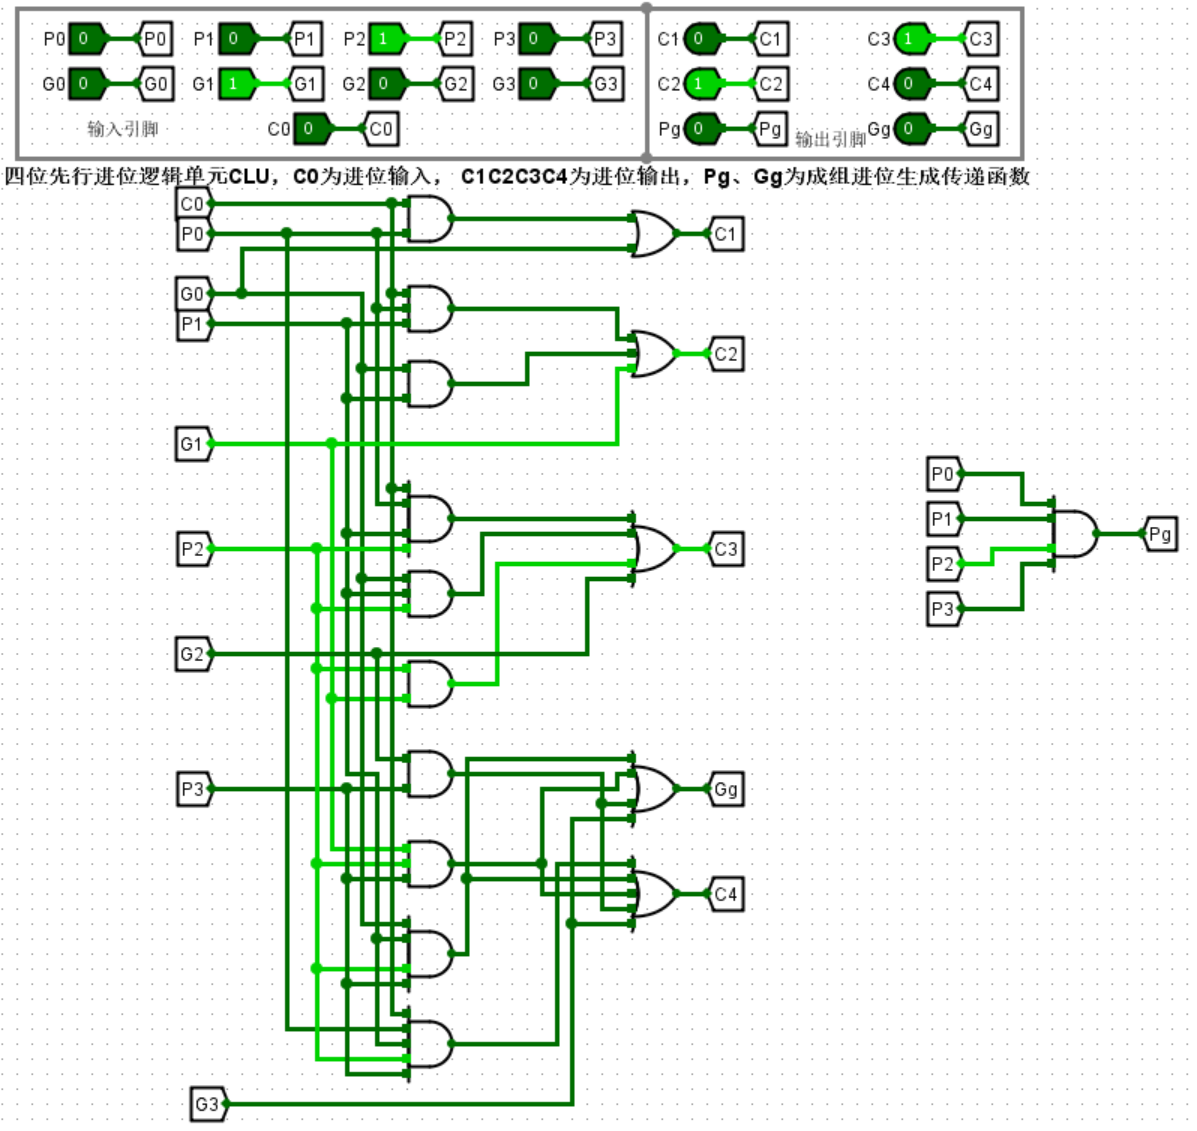
\includegraphics[width=0.4\textwidth]{1.5.1.png}
    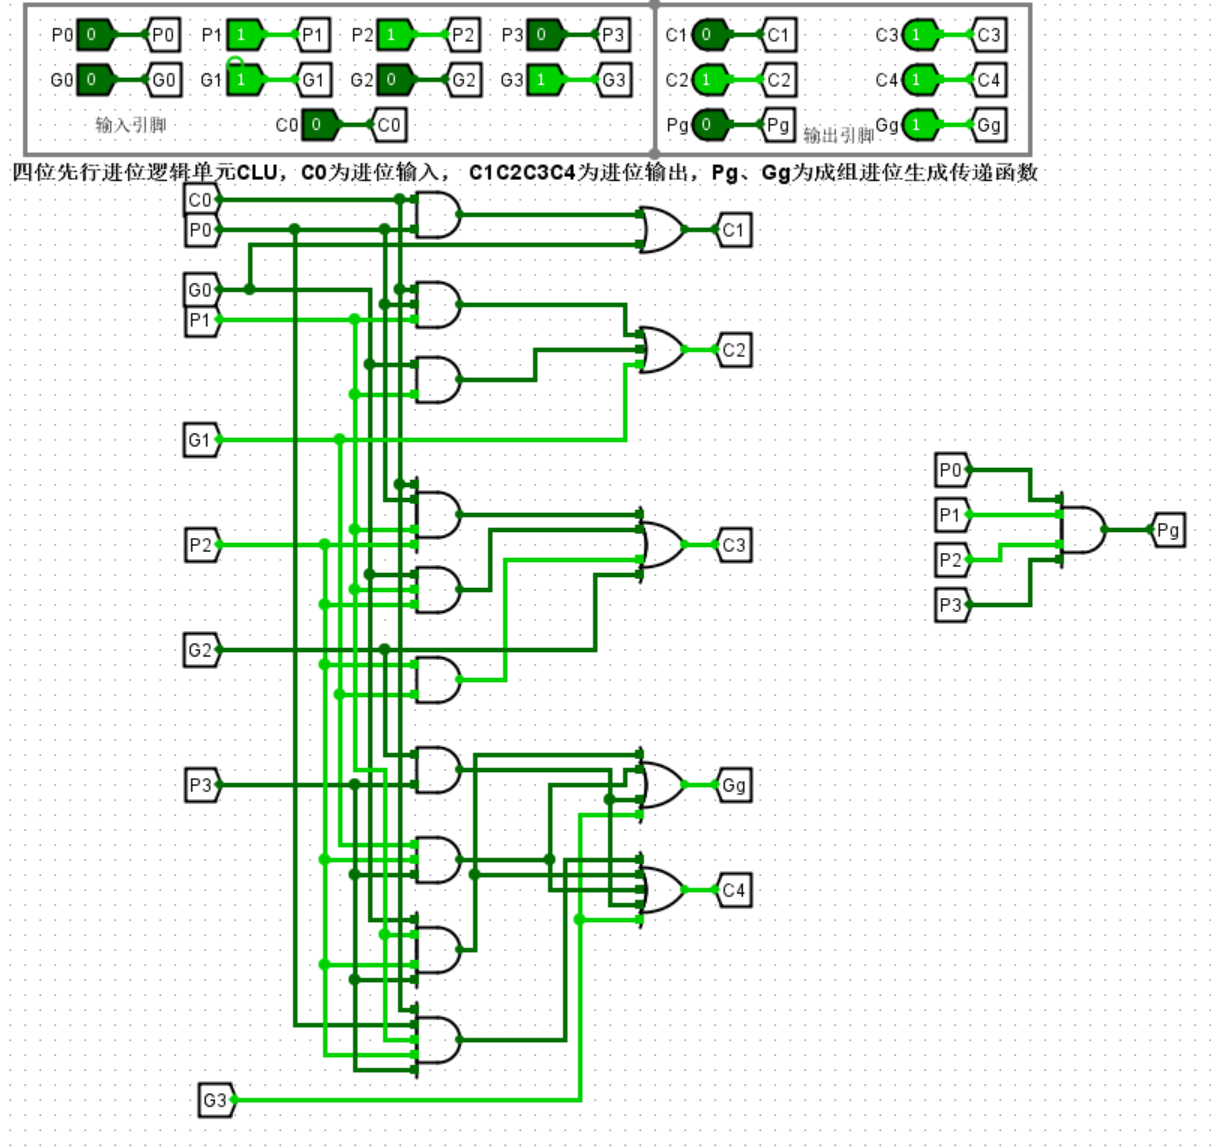
\includegraphics[width=0.4\textwidth]{1.5.2.png}
    
    \caption{CLU仿真测试图}
    \end{figure}

    \begin{figure}[H]
    \centering
    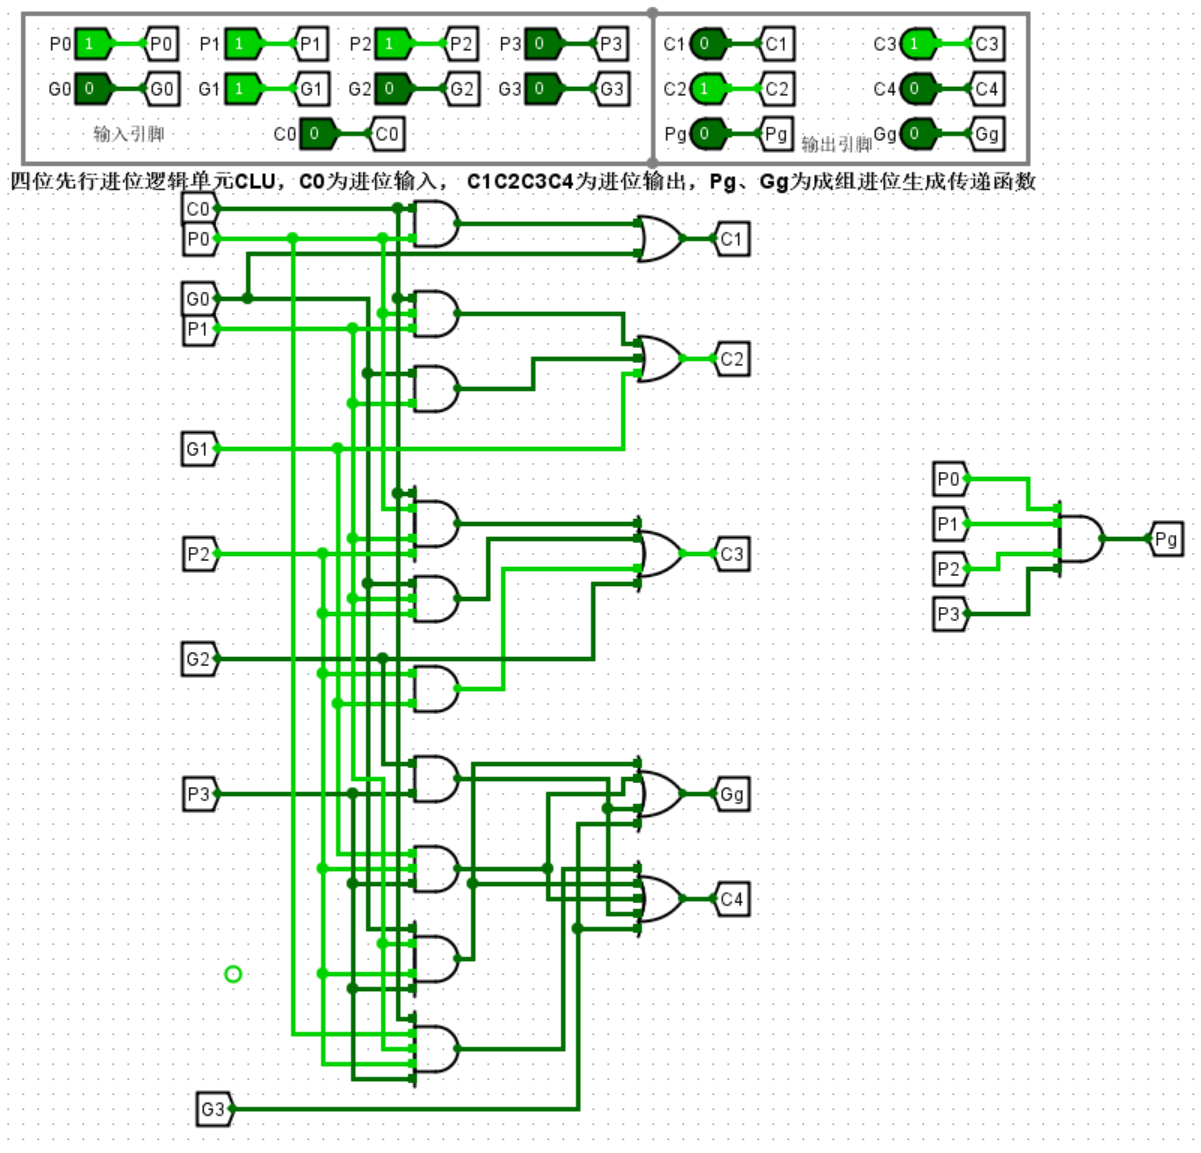
\includegraphics[width=0.4\textwidth]{1.5.3.png}  
    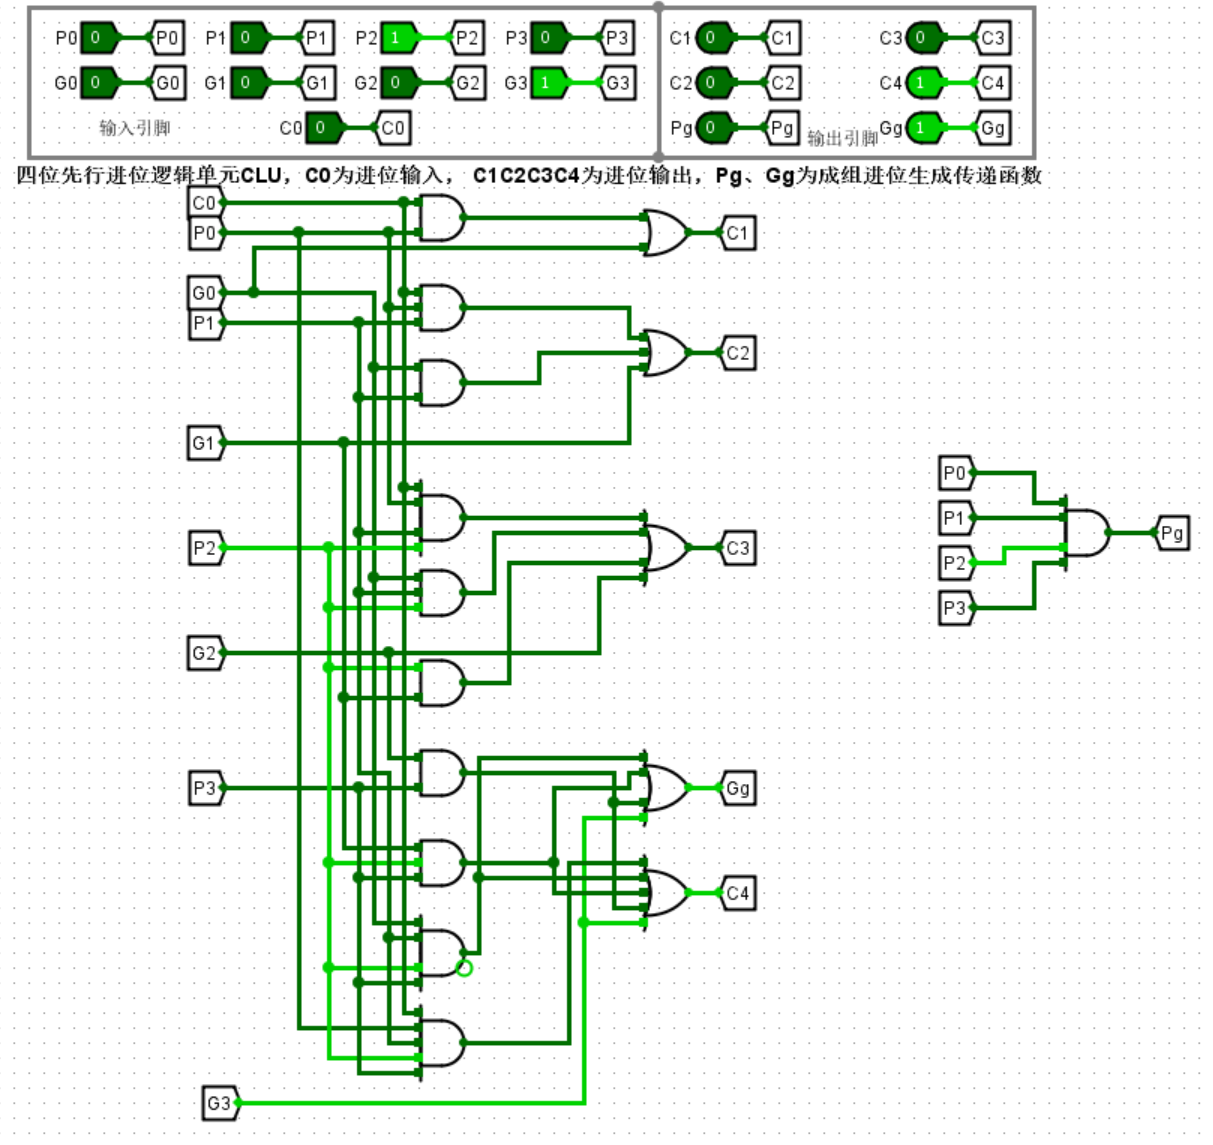
\includegraphics[width=0.4\textwidth]{1.5.4.png}
    \caption{CLU仿真测试图}
    \end{figure}
    
    
    逻辑表达式如下,仿真结果均正确。
    
    $\begin{aligned}
        &C_1 =G_0 + P_0 C_0  \\
        &C_2 =G_1+P_1G_0+P_1P_0C_0  \\
        &C_3 =G_2+P_2G_1+P_2P_1G_0+P_2P_1P_0C_0  \\
        &C_4 =G_3+P_3G_2+P_3P_2G_1+P_3P_2P_1G_0+P_3P_2P_1P_0C_0  \\
        &P_g =P_3P_2P_1P_0  \\
        &G_g =G_3+P_3G_2+P_3P_2G_1+P_3P_2P_1G_0 
    \end{aligned}$

    \subsubsection{错误现象及分析}
    在完成实验的过程中,没有遇到任何错误。

    \subsection{4位快速加法器 CLA}

    \subsubsection{整体方案设计}
    \begin{figure}[H]
    \centering
    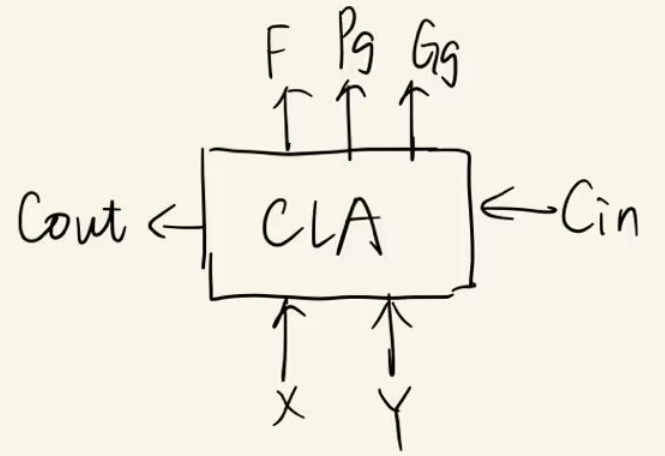
\includegraphics[width=0.4\textwidth]{2.1.png}
    \caption{4位快速加法器CLA整体方案设计}
    \end{figure}

    \subsubsection{顶层模块设计}
    实验电路较为简单,不需要顶层模块设计图。

    \subsubsection{引脚作用}
    \begin{table}[H]
    \centering
    \begin{tabular}{|c|c|}
        \hline
        $Cin$  & 输入的最低位进位 \\ \hline
        $X_{0}\thicksim X_{3}$ & 输入的四位加数 \\ \hline
        $Y_{0}\thicksim Y_{3}$   & 输入的四位被加数 \\ \hline
        $F_{0}\thicksim F_{3}$   & 输出的四位和 \\ \hline
        $Cout$   & 输出的最高位进位 \\ \hline
        $P_{g}$   & 输入的组间进位传递函数 \\ \hline
        $G_{g}$   & 输出的组间进位生成函数 \\ \hline
    \end{tabular}
    \caption{CLA引脚作用}
    \end{table}

    \subsubsection{原理图和电路图}
    \begin{figure}[H]
    \centering
    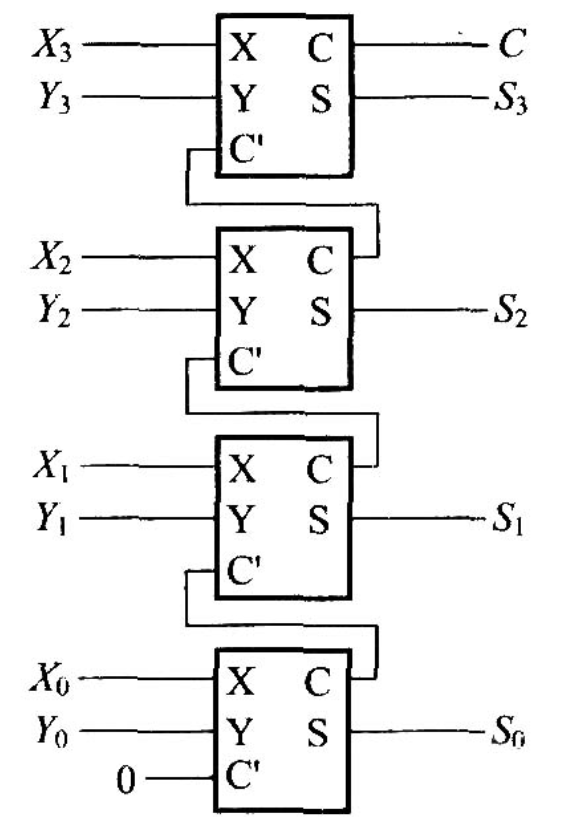
\includegraphics[width=0.4\textwidth]{2.4.1.png}
    \caption{CLA原理图}
    \end{figure}

    \begin{figure}[H]
    \centering
    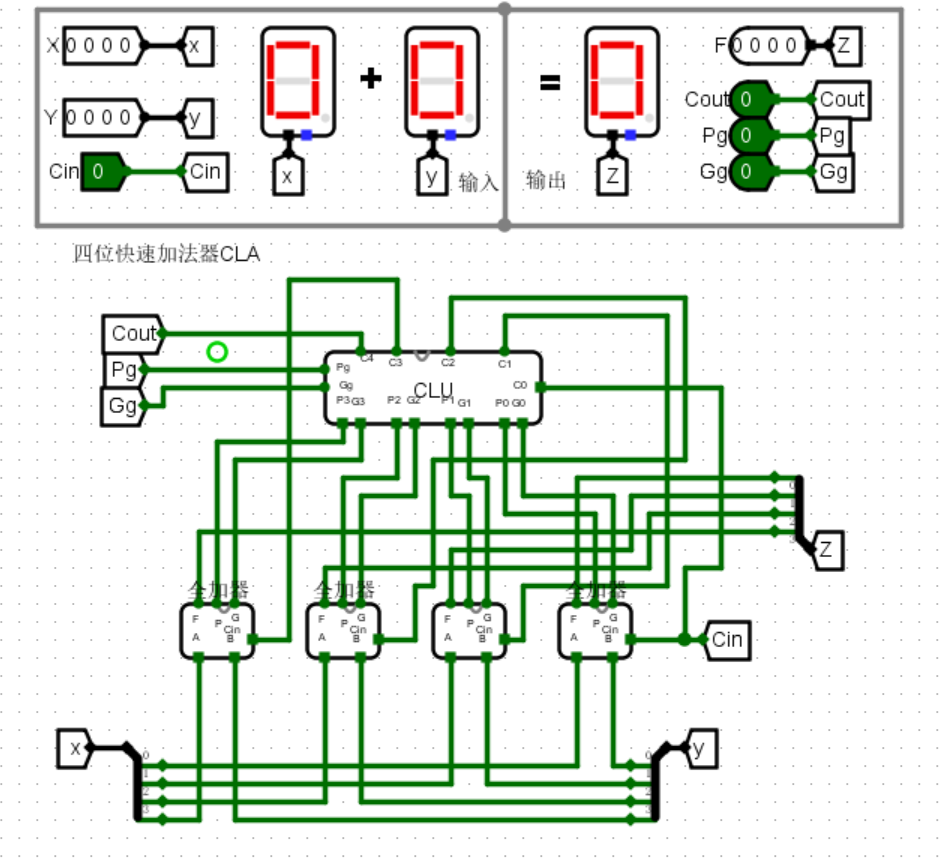
\includegraphics[width=0.8\textwidth]{2.4.2.png}
    \caption{CLA电路图}
    \end{figure}

    \subsubsection{仿真测试图}
    \begin{figure}[H]
    \centering
    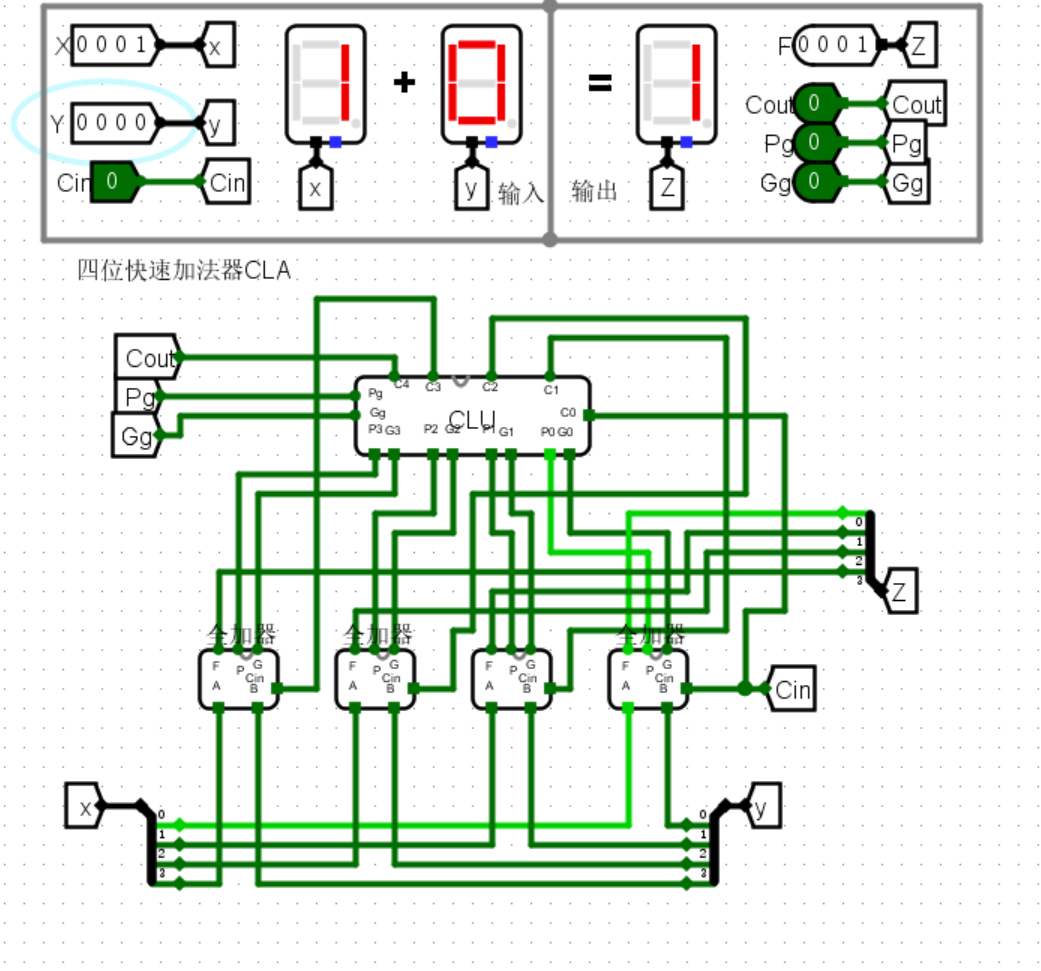
\includegraphics[width=0.4\textwidth]{2.5.1.png}
    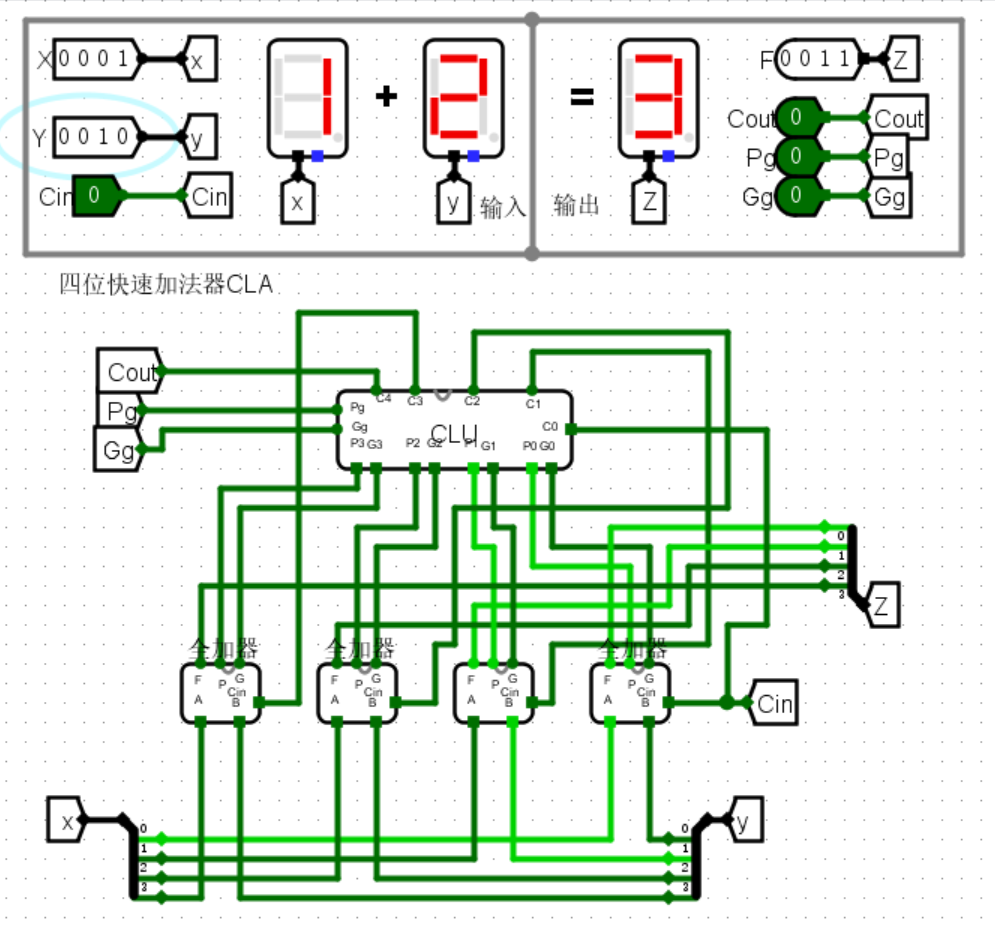
\includegraphics[width=0.4\textwidth]{2.5.2.png}
    \caption{CLA仿真测试图}
    \end{figure}

    \begin{figure}[H]
    \centering
    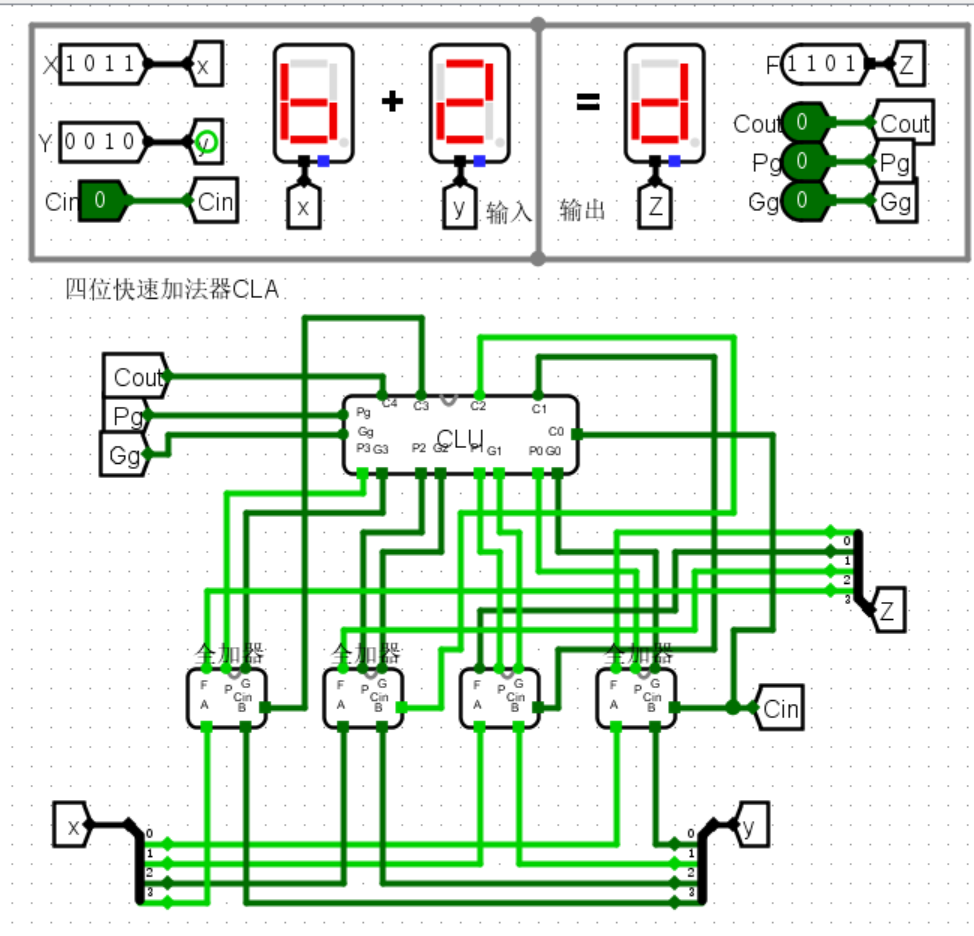
\includegraphics[width=0.4\textwidth]{2.5.3.png}
    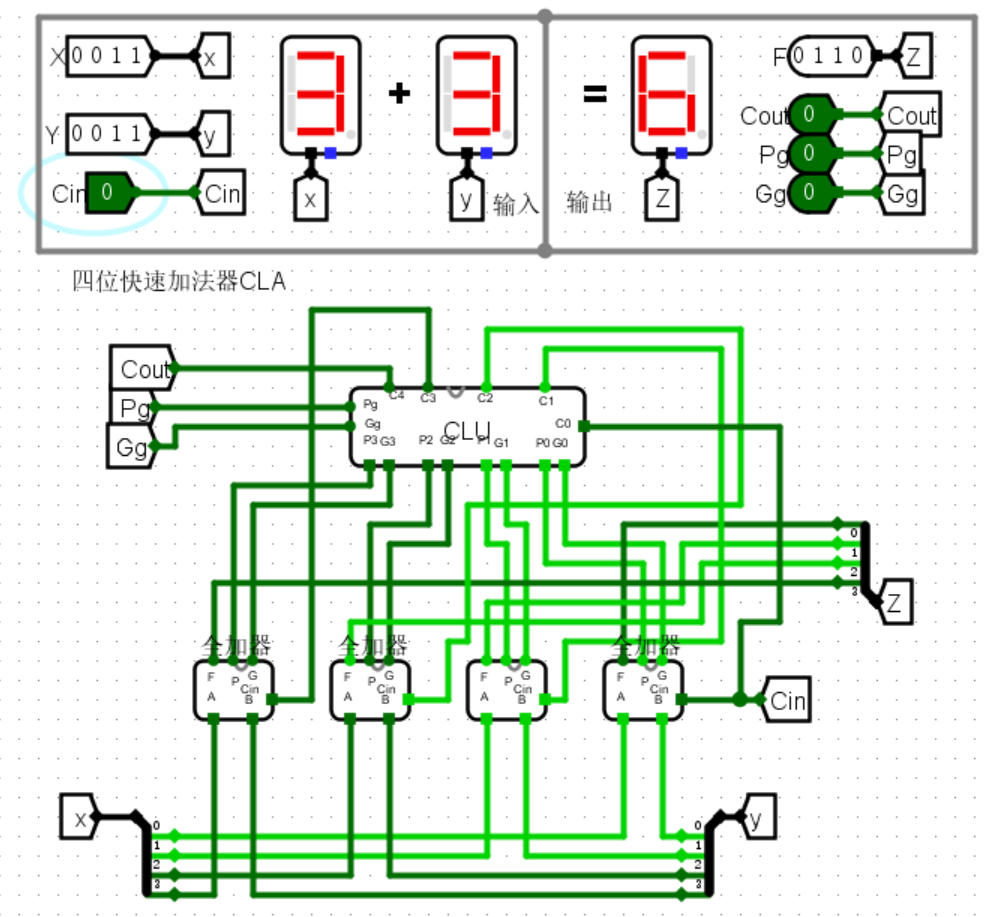
\includegraphics[width=0.4\textwidth]{2.5.4.png}
    \caption{CLA仿真测试图}
    \end{figure}

    显然仿真结果全部正确。

    \subsubsection{错误现象及分析}
    在完成实验的过程中,没有遇到任何错误。

    \subsection{16位两级先行进位加法器}

    \subsubsection{整体方案设计}
    \begin{figure}[H]
    \centering
    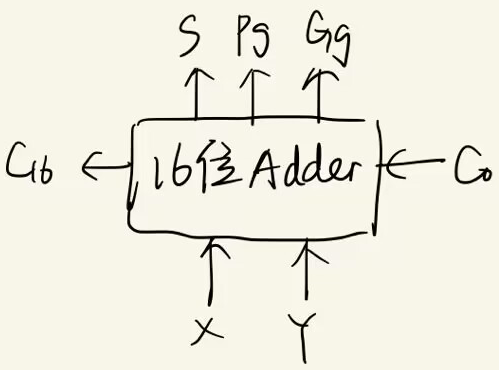
\includegraphics[width=0.4\textwidth]{3.1.png}
    \caption{16位两级先行进位加法器整体方案设计}
    \end{figure}

    \subsubsection{顶层模块设计}
    实验电路较为简单,不需要顶层模块设计图。

    \subsubsection{引脚作用}
    \begin{table}[H]
    \centering
    \begin{tabular}{|c|c|}
        \hline
        $C_{0}$  & 输入的最低位进位 \\ \hline
        $X_{0}\thicksim X_{15}$ & 输入的十六位加数 \\ \hline
        $Y_{0}\thicksim Y_{15}$   & 输入的十六位被加数 \\ \hline
        $S_{0}\thicksim S_{15}$   & 输出的十六位和 \\ \hline
        $Cout$   & 输出的最高位进位 \\ \hline
        $P_{g}$   & 输入的组间进位传递函数 \\ \hline
        $G_{g}$   & 输出的组间进位生成函数 \\ \hline
    \end{tabular}
    \caption{16位两级先行进位加法器引脚作用}
    \end{table}

    \subsubsection{原理图和电路图}
    \begin{figure}[H]
    \centering
    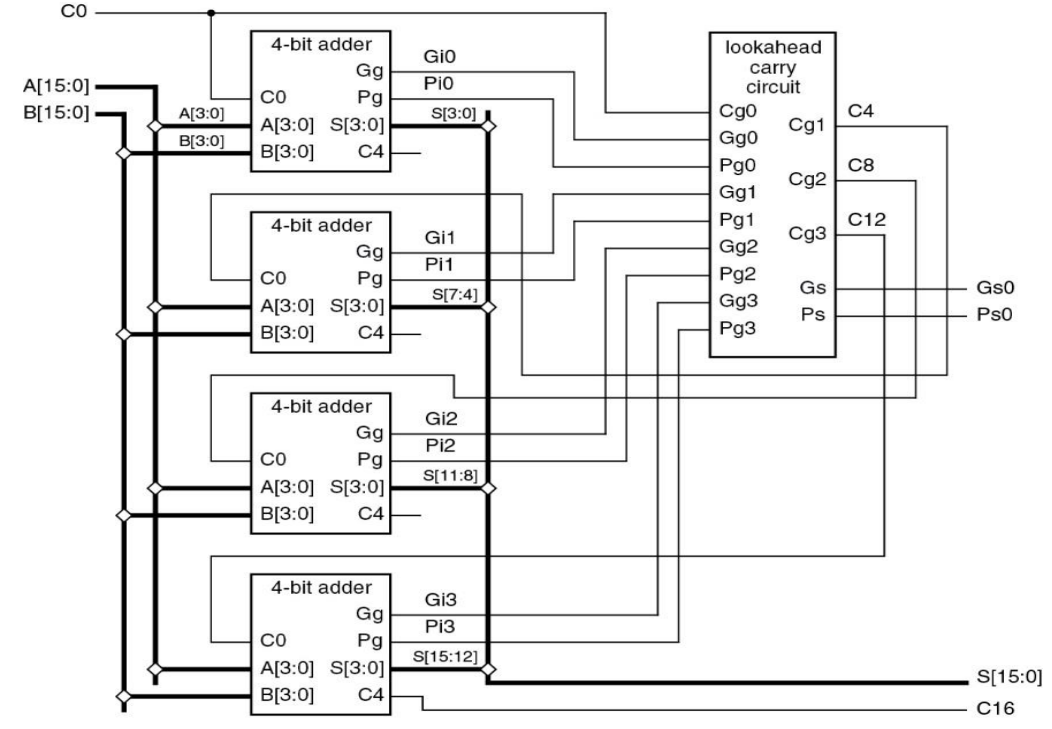
\includegraphics[width=0.8\textwidth]{3.4.1.png}
    \caption{16位两级先行进位加法器原理图}
    \end{figure}

    \begin{figure}[H]
    \centering
    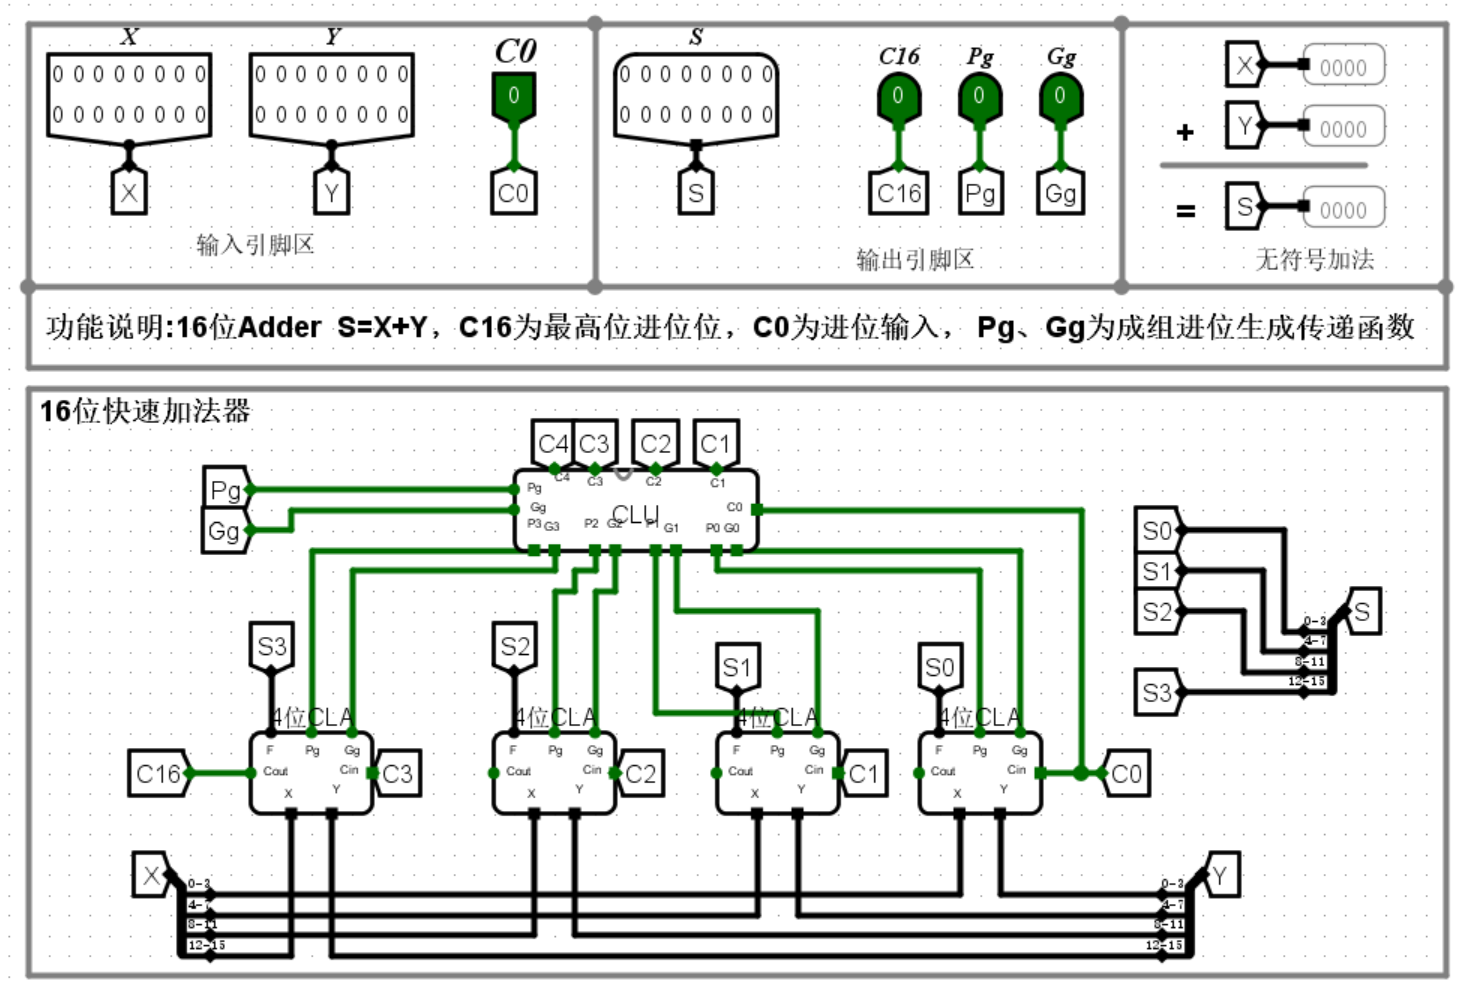
\includegraphics[width=0.8\textwidth]{3.4.2.png}
    \caption{16位两级先行进位加法器电路图}
    \end{figure}

    \subsubsection{仿真测试图}
    \begin{figure}[H]
    \centering
    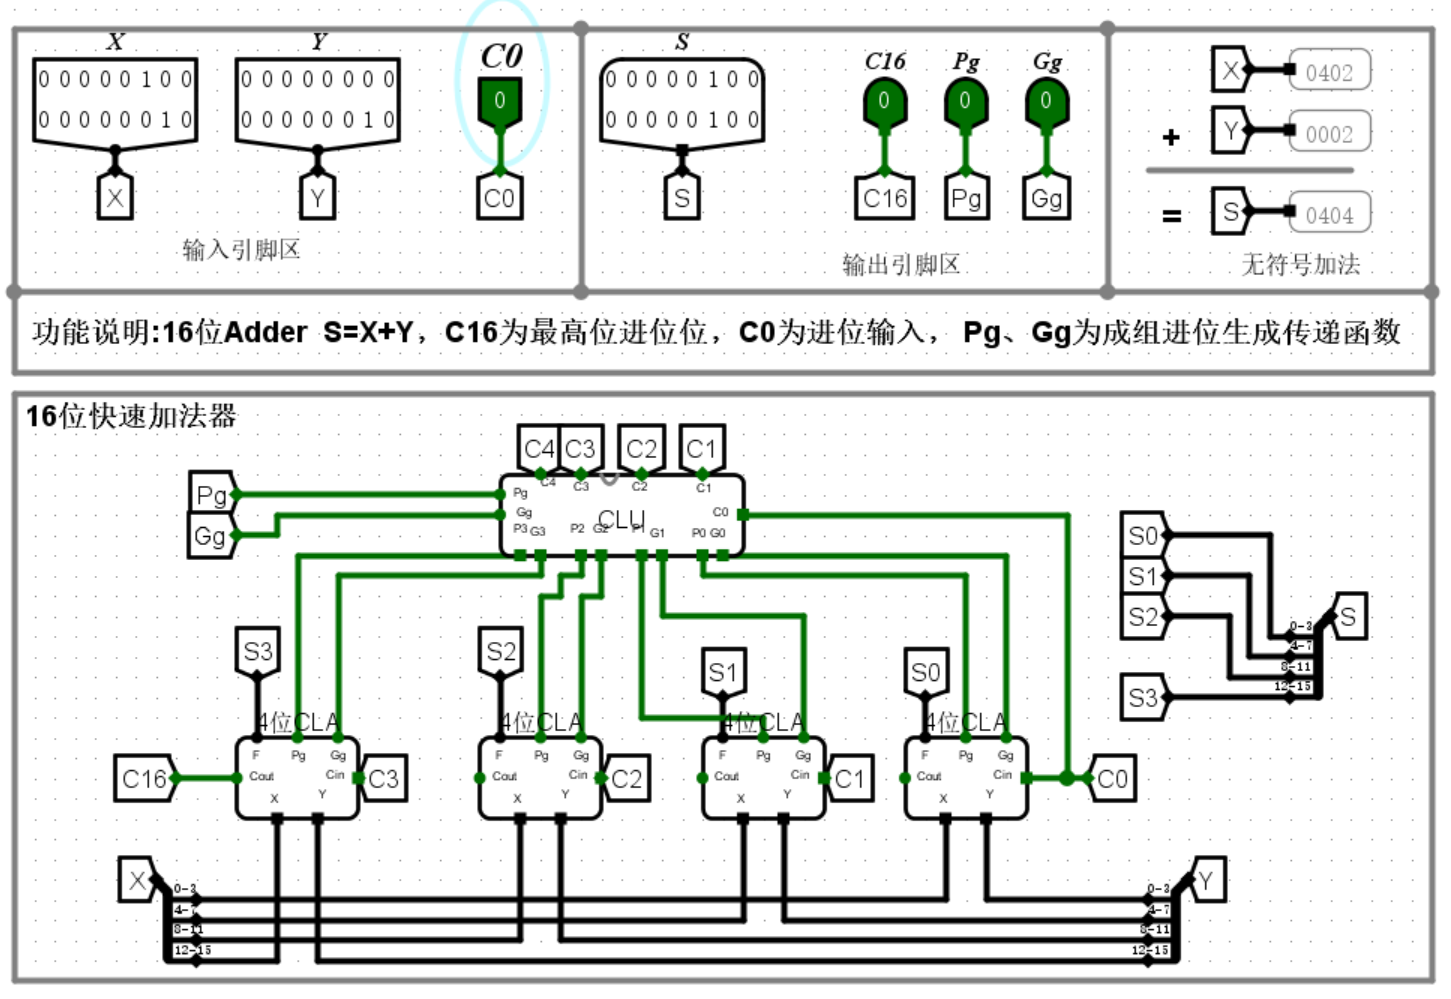
\includegraphics[width=0.4\textwidth]{3.5.1.png}
    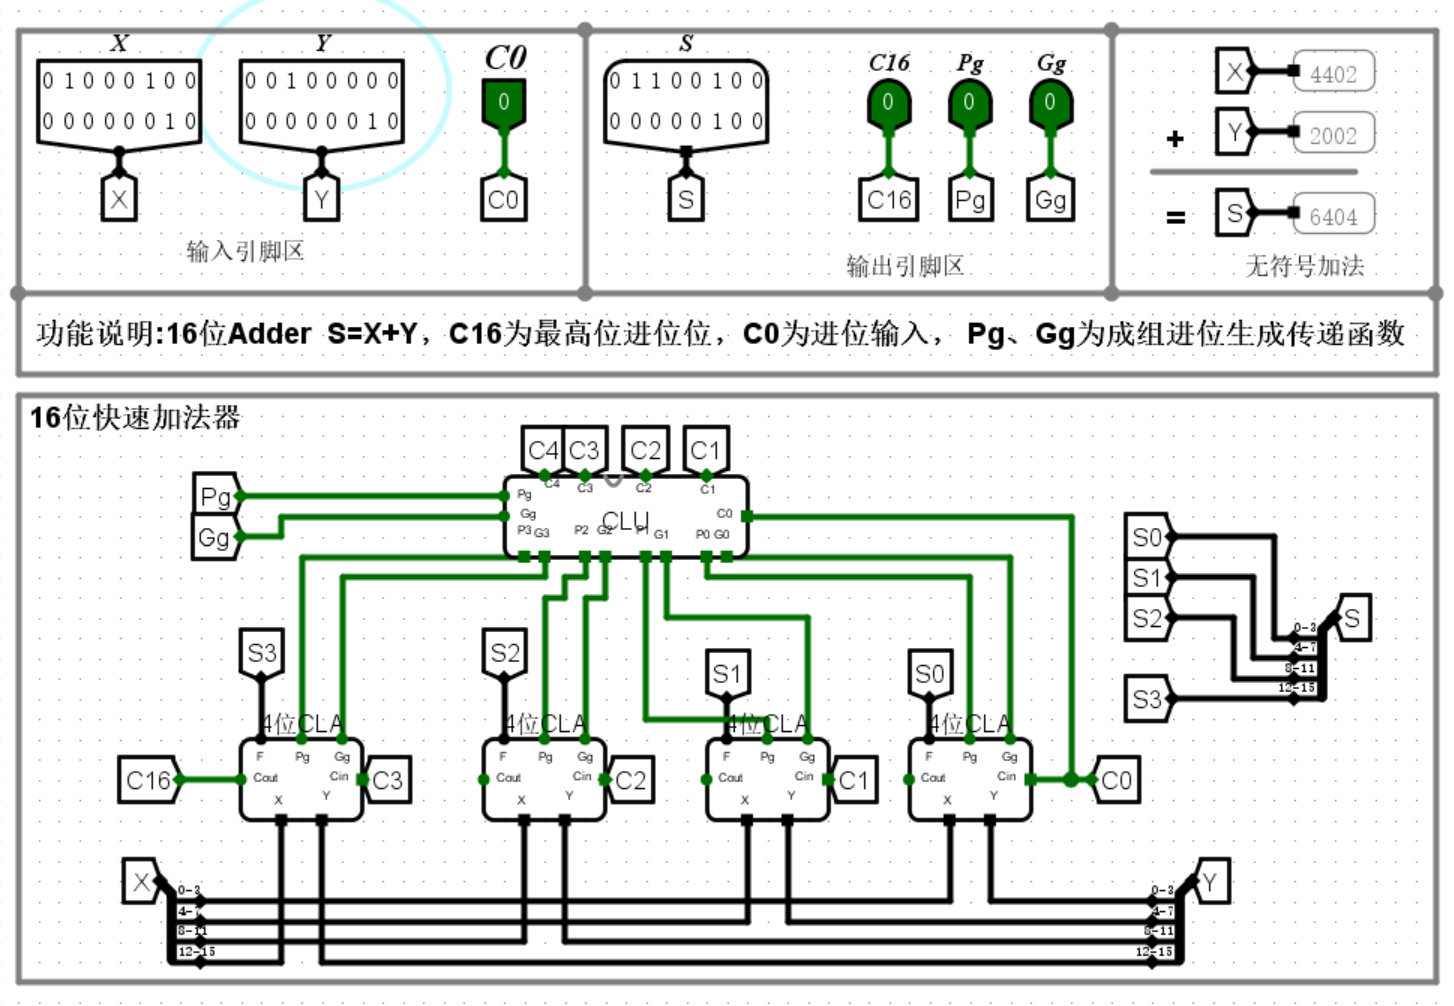
\includegraphics[width=0.4\textwidth]{3.5.2.png}
    \caption{16位两级先行进位加法器仿真测试图}
    \end{figure}

    \begin{figure}[H]
    \centering
    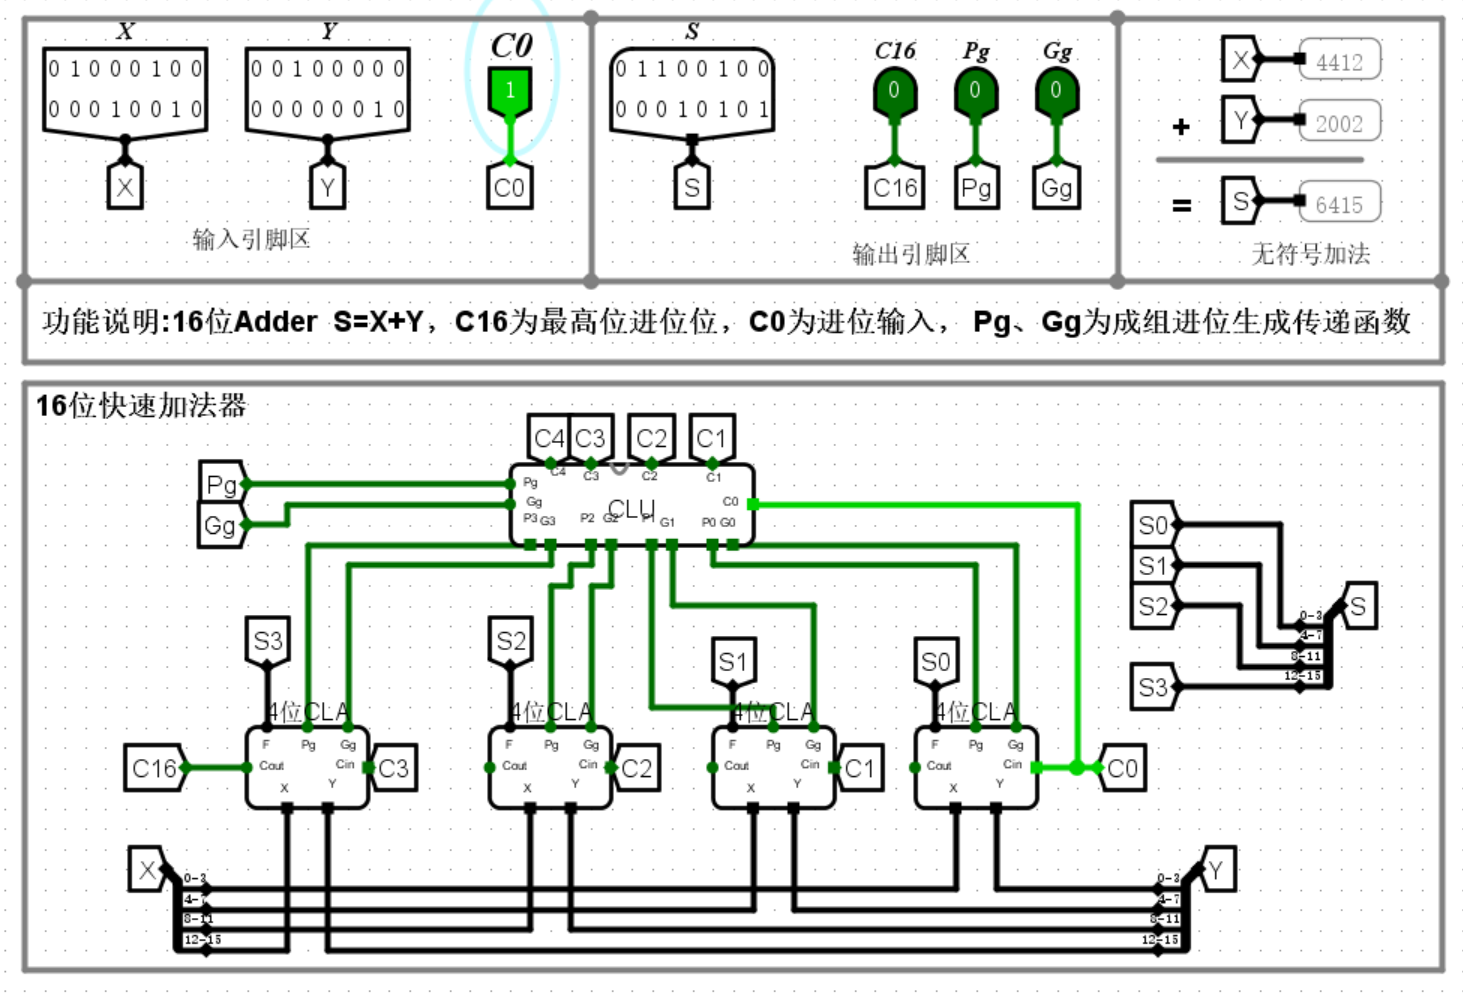
\includegraphics[width=0.4\textwidth]{3.5.3.png}
    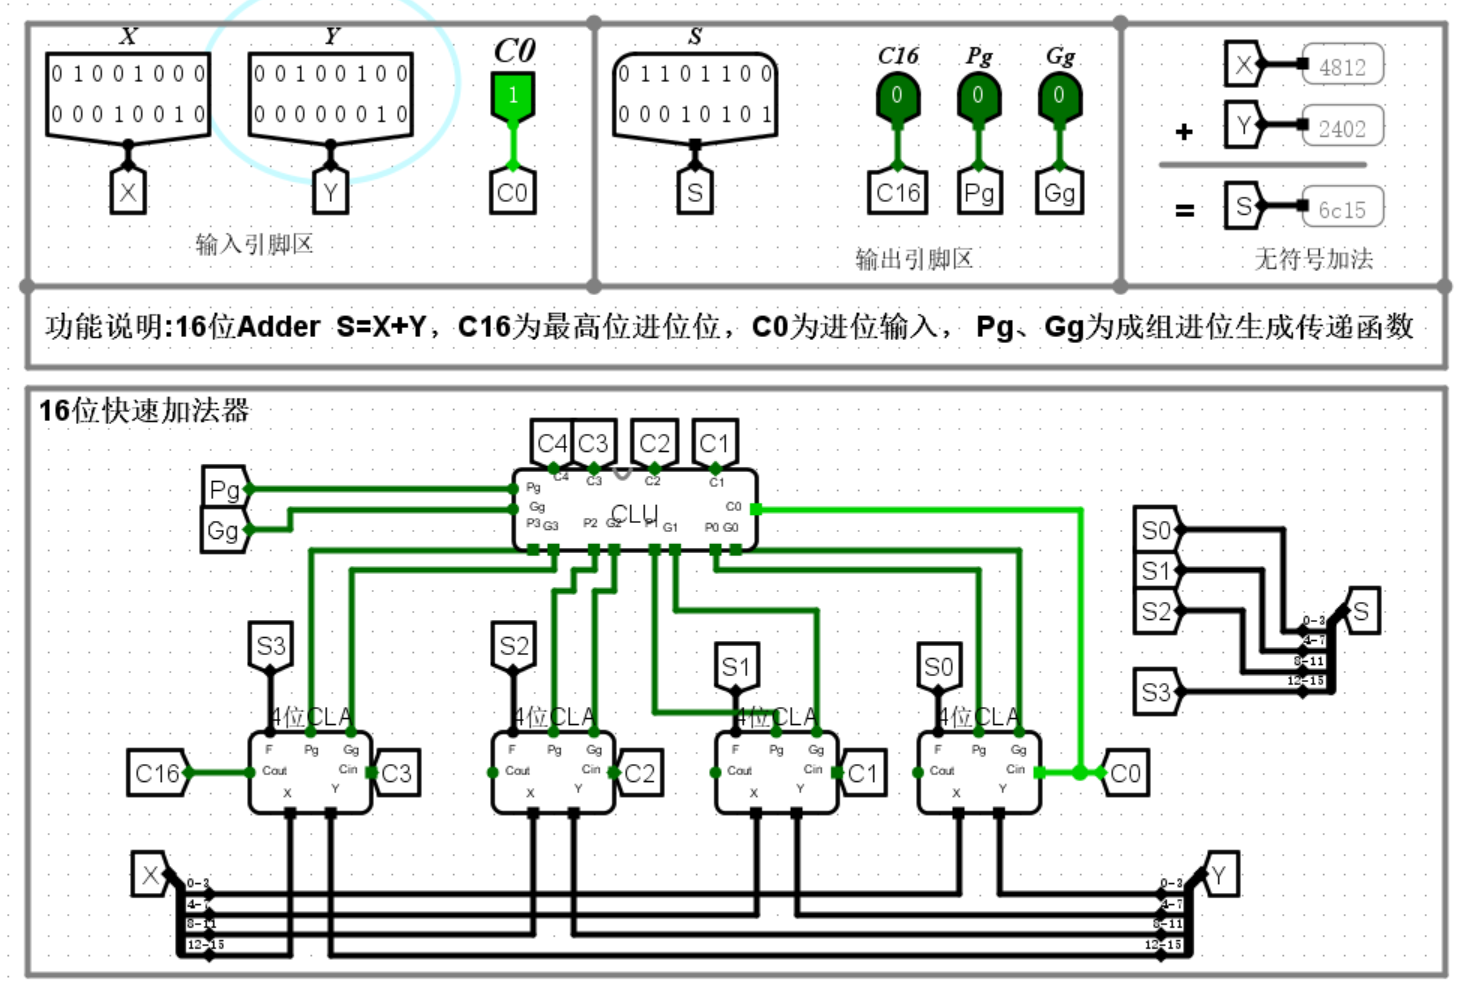
\includegraphics[width=0.4\textwidth]{3.5.4.png}
    \caption{16位两级先行进位加法器仿真测试图}
    \end{figure}

    0402H+0002H=0404H;\\
    4402H+2002H=6404H;\\
    4412H+2002H=6415H;($C_{0}=1$)\\
    4812H+2402H=6c15H;($C_{0}=1$)\\
    \subsubsection{错误现象及分析}
    在完成实验的过程中,没有遇到任何错误。
    
    \subsection{32位加法器}\
    \subsubsection{整体方案设计}
    \begin{figure}[H]
    \centering
    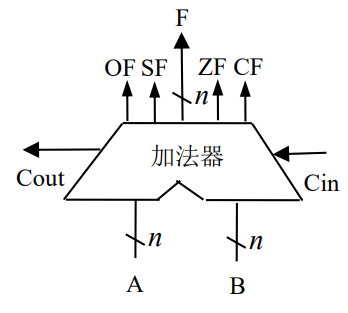
\includegraphics[width=0.4\textwidth]{4.1.png}
    \caption{32位加法器整体方案设计}
    \end{figure}

    \subsubsection{顶层模块设计}
    实验电路较为简单,不需要顶层模块设计图。
    \subsubsection{引脚作用}
    \begin{table}[H]
    \centering
    \begin{tabular}{|c|c|}
        \hline
        $C_{0}$  & 输入的最低位进位 \\ \hline
        $X_{0}\thicksim X_{31}$ & 输入的三十二位加数 \\ \hline
        $Y_{0}\thicksim Y_{31}$   & 输入的三十二位被加数 \\ \hline
        $S_{0}\thicksim S_{31}$   & 输出的三十二位和 \\ \hline
        $Cout$   & 输出的最高位进位 \\ \hline
        $OF$   & 输出的溢出标志 \\ \hline
        $CF$   & 输出的进/借位标志 \\ \hline
        $ZF$   & 输出的零标志 \\ \hline
        $SF$   & 输出的符号标志 \\ \hline
    \end{tabular}
    \caption{32位加法器引脚作用}
    \end{table}

    \subsubsection{原理图和电路图}
    \begin{figure}[H]
    \centering
    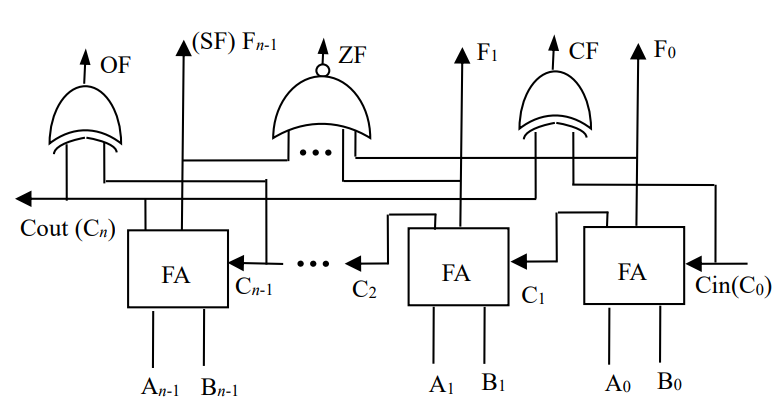
\includegraphics[width=0.8\textwidth]{4.4.1.png}
    \caption{32位加法器原理图}
    \end{figure}

    \begin{figure}[H]
    \centering
    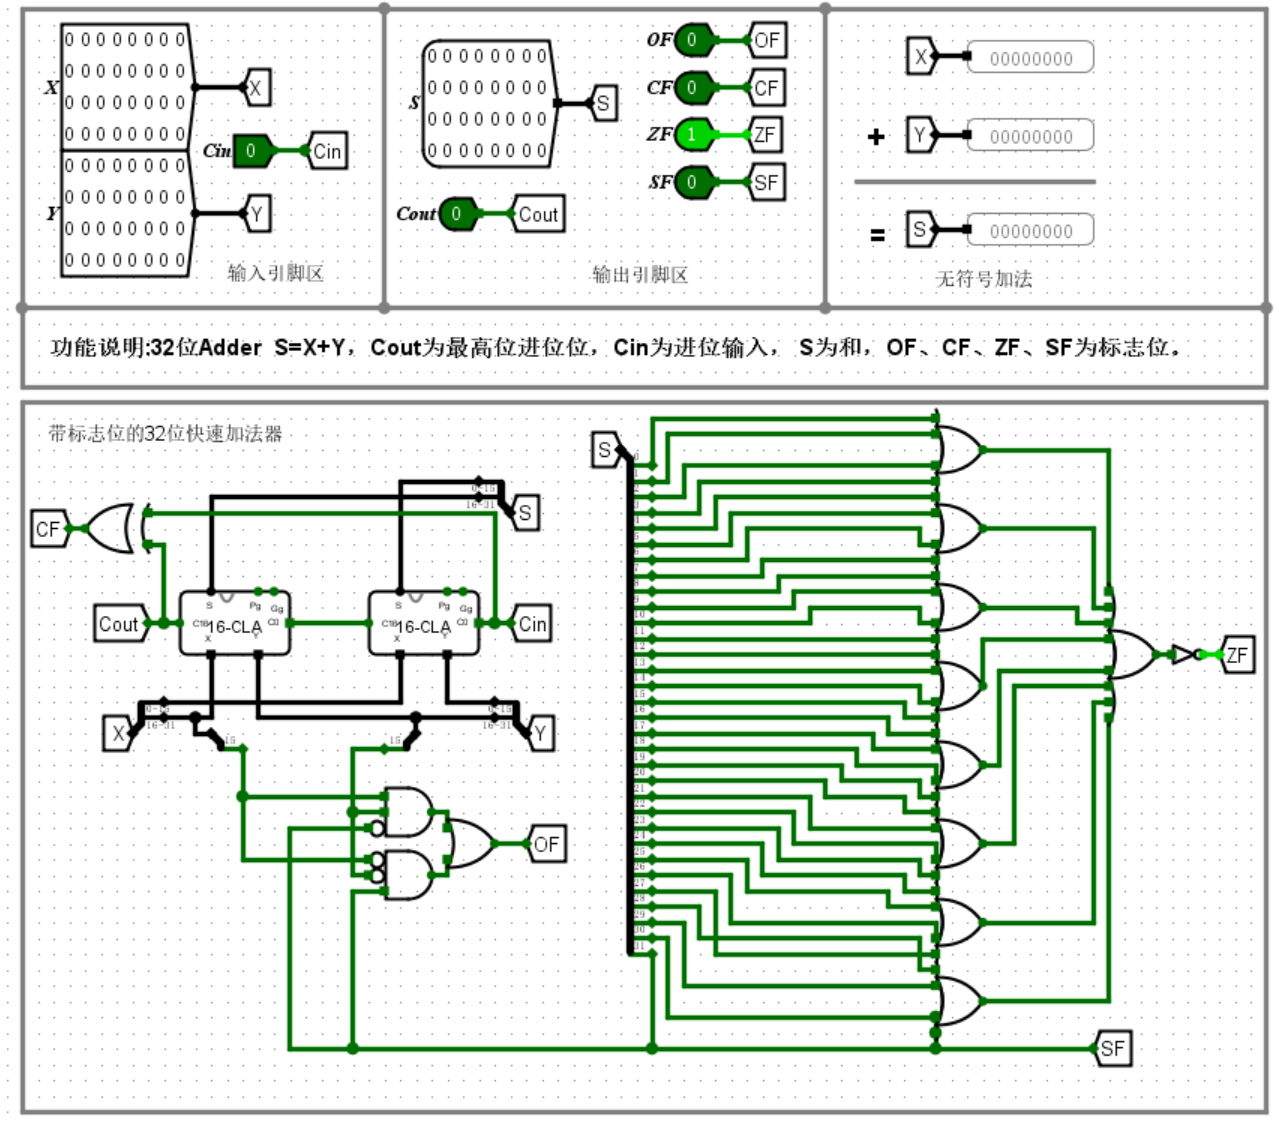
\includegraphics[width=0.8\textwidth]{4.4.2.png}
    \caption{32位加法器电路图}
    \end{figure}

    \subsubsection{仿真测试图}
    \begin{figure}[H]
    \centering
    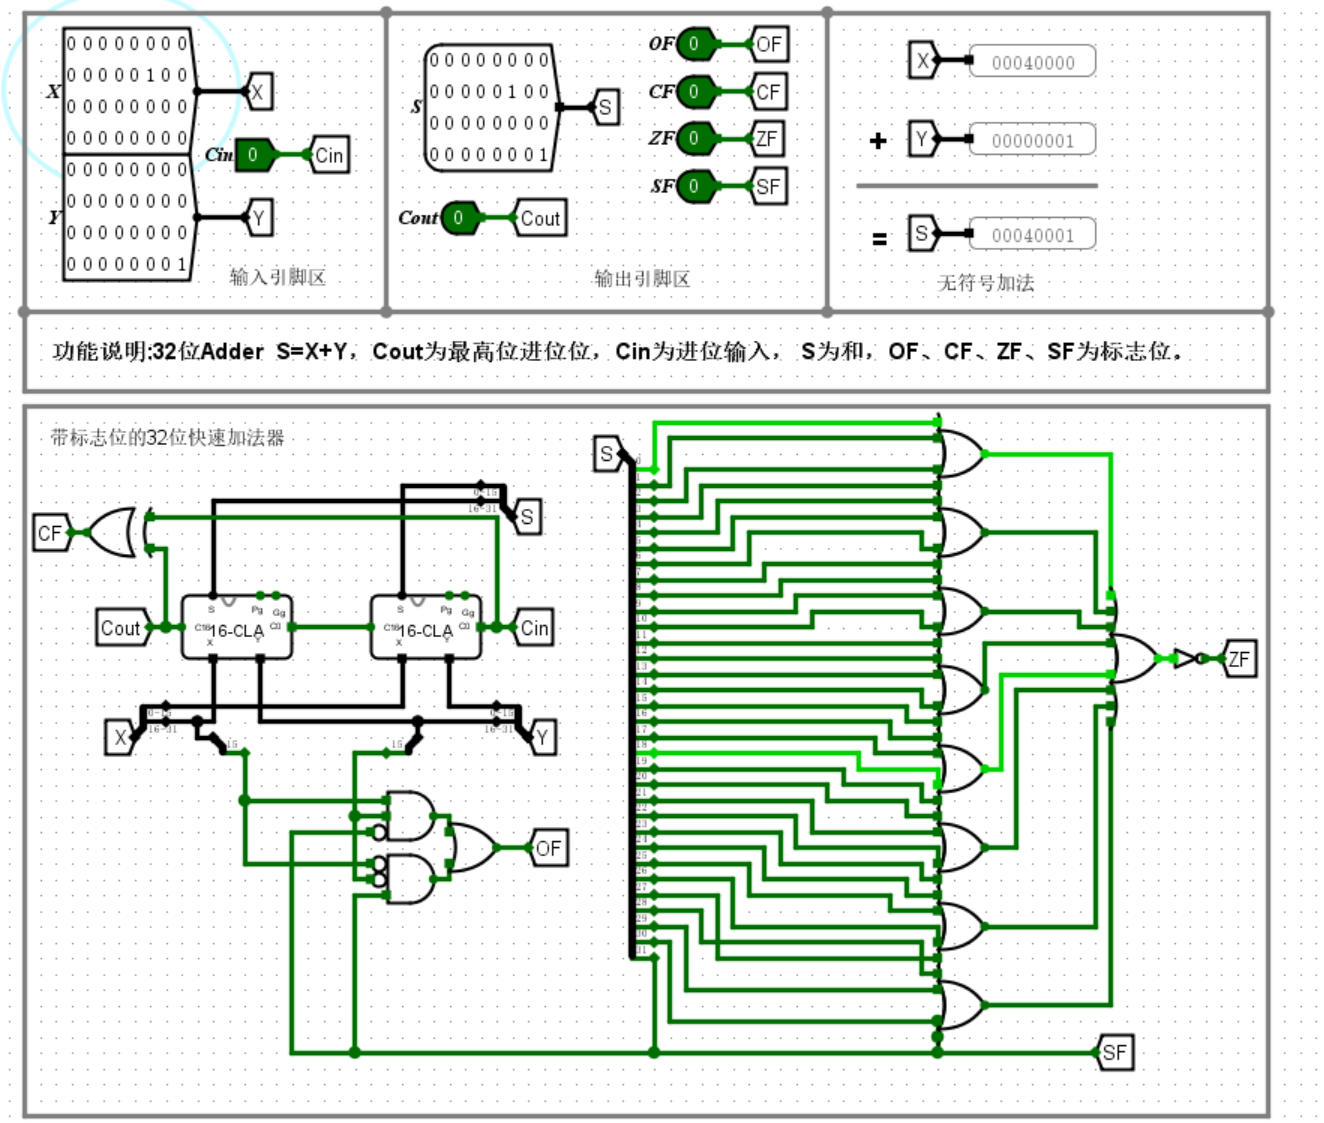
\includegraphics[width=0.4\textwidth]{4.5.1.png}
    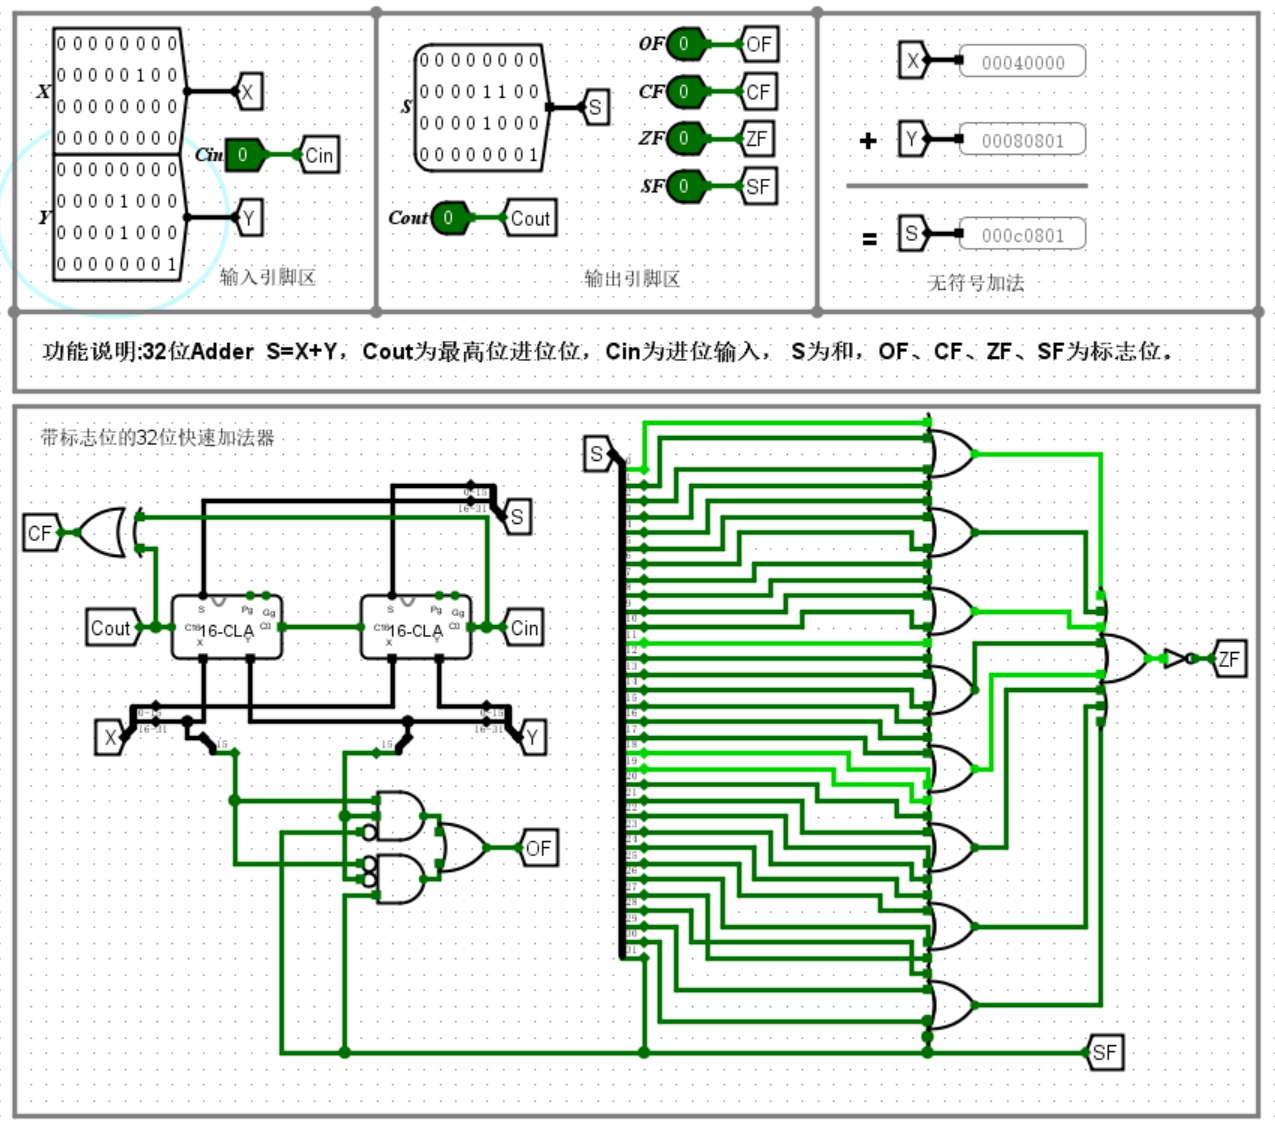
\includegraphics[width=0.4\textwidth]{4.5.2.png}
    \caption{32位加法器仿真测试图}
    \end{figure}

    \begin{figure}[H]
    \centering
    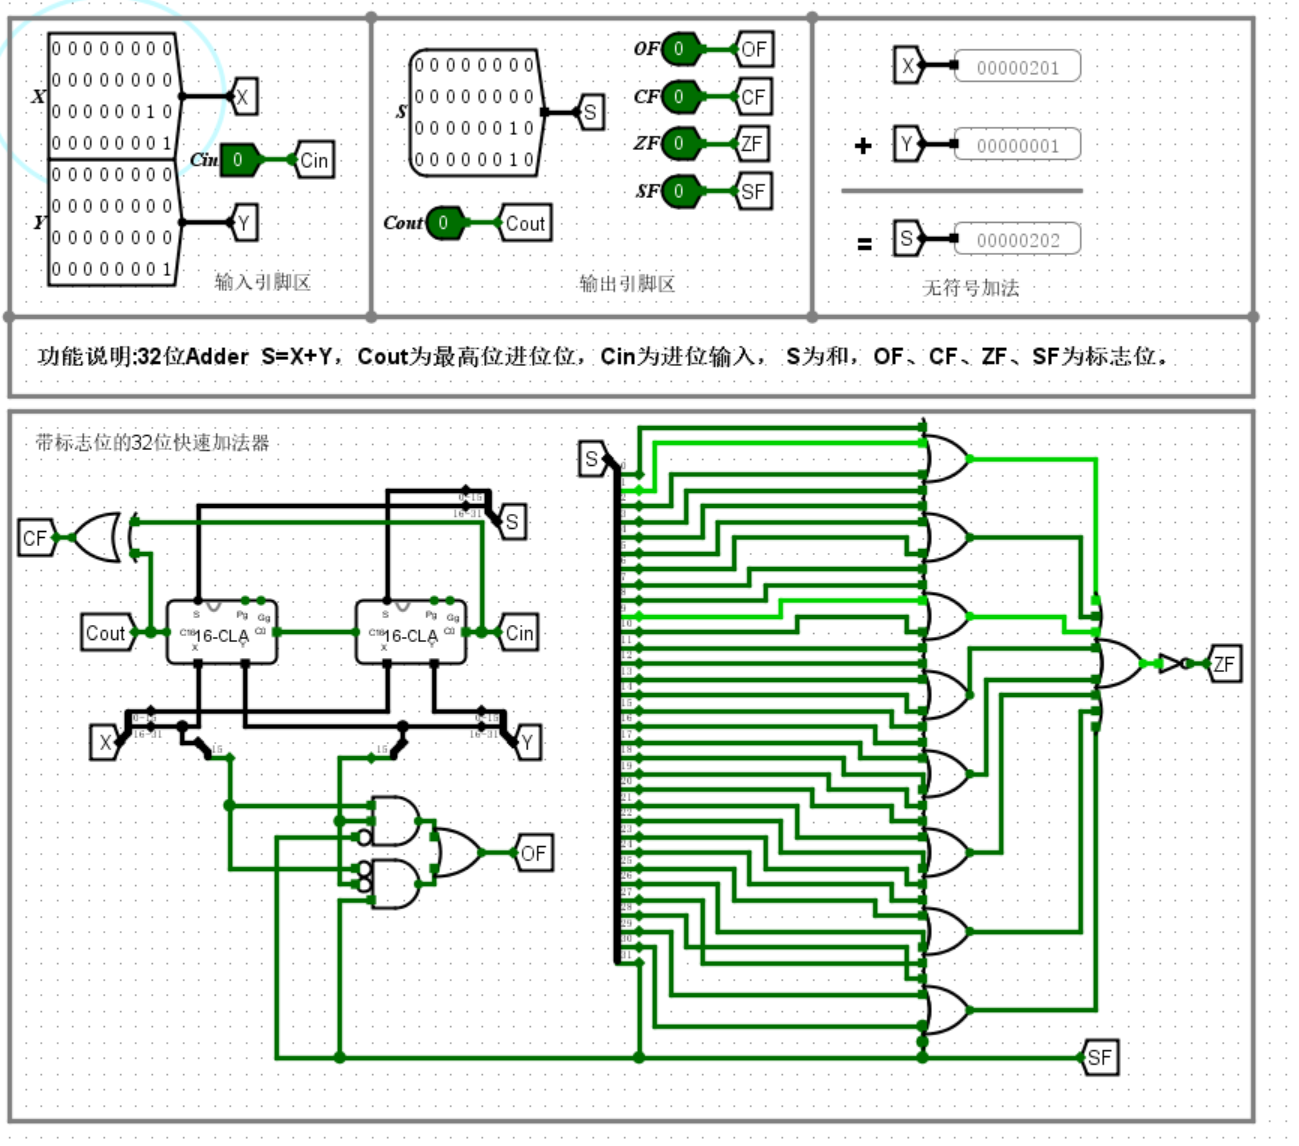
\includegraphics[width=0.4\textwidth]{4.5.3.png}
    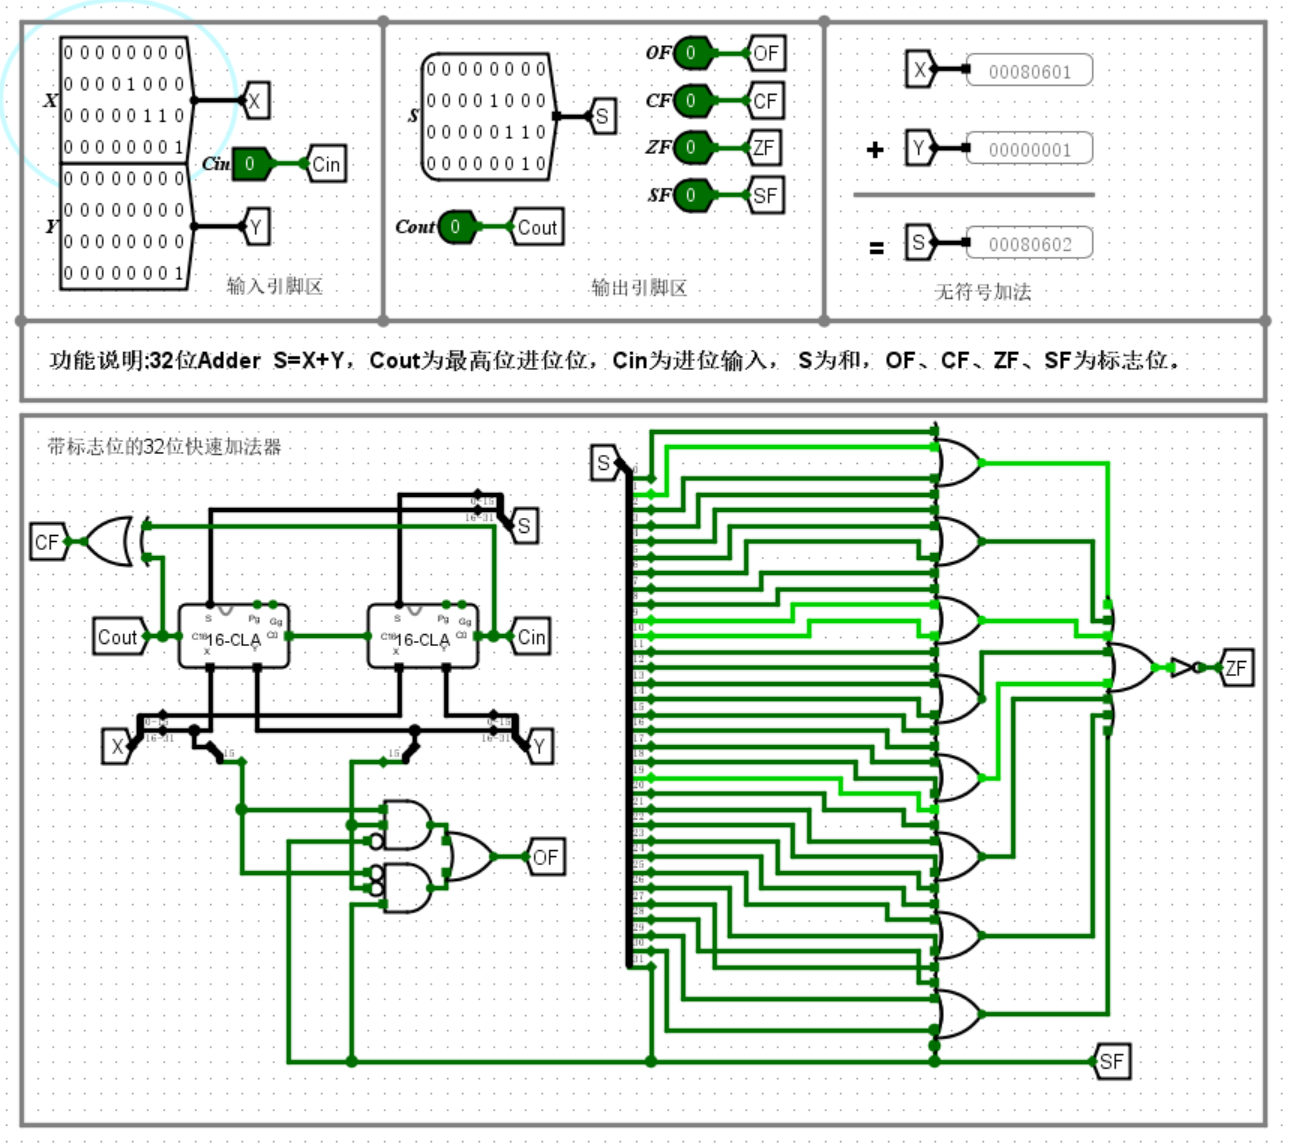
\includegraphics[width=0.4\textwidth]{4.5.4.png}
    \caption{32位加法器仿真测试图}
    \end{figure}

    00040000H+00000001H=00004001H;\\
    00040000H+00080801H=000c0801H;\\
    00000201H+00000001H=00000202H;\\
    00080601H+00000001H=00080602H;\\
    标志位的逻辑表达式为
    $\begin{aligned}
        &OF =\overline{X_{n-1}}\cdot\overline{Y_{n-1}}\cdot S_{n-1}+X_{n-1}\cdot Y_{n-1}\cdot\overline{S_{n-1}}  \\
        &CF =Cin\oplus Cout  \\
        &ZF =\overline{S_{n-1}+S_{n-2}+\cdots+S_0}  \\
        &SF =S_{n-1} 
    \end{aligned}$
    
    \subsubsection{错误现象及分析}
    在完成实验的过程中,没有遇到任何错误。

    \subsection{ALU操作控制信号生成部件}
    \subsubsection{整体方案设计}
    \begin{figure}[H]
    \centering
    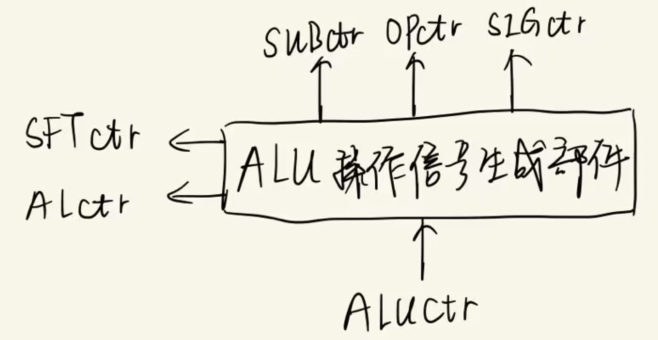
\includegraphics[width=0.4\textwidth]{5.1.png}
    \caption{ALU操作控制信号生成部件整体方案设计}
    \end{figure}

    \subsubsection{顶层模块设计}
    实验电路较为简单,不需要顶层模块设计图。
    \subsubsection{引脚作用}
    \begin{table}[H]
    \centering
    \begin{tabular}{|c|c|}
        \hline
        ALUctr[3:0]   & 输入的 ALU 控制信号 \\ \hline
        SUBctr & 输出的 SUB 控制信号 \\ \hline
        SIGctr   & 输出的 SIG 控制信号 \\ \hline
        SFTctr   & 输出的 SFT 控制信号 \\ \hline
        ALctr  & 输出的 AL 控制信号 \\ \hline
        OPctr[3:0]  & 输出的 OP 控制信号 \\ \hline
    \end{tabular}
    \caption{ALU操作控制信号生成部件引脚作用}
    \end{table}

    \subsubsection{原理图和电路图}
    \begin{figure}[H]
    \centering
    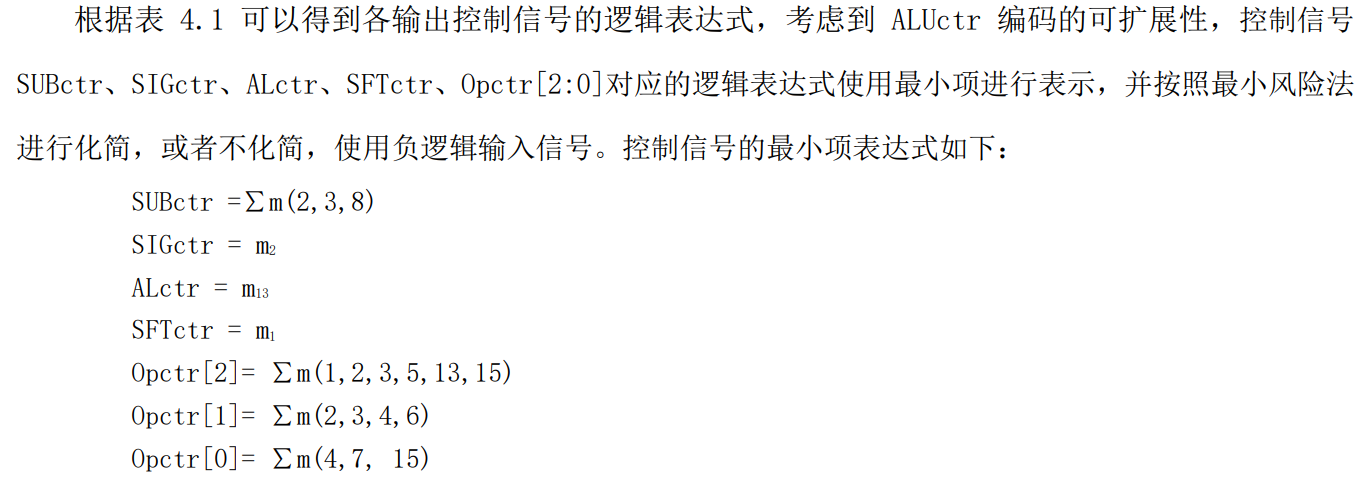
\includegraphics[width=0.8\textwidth]{5.4.1.png}
    \caption{ALU操作控制信号生成部件原理图}
    \end{figure}

    \begin{figure}[H]
    \centering
    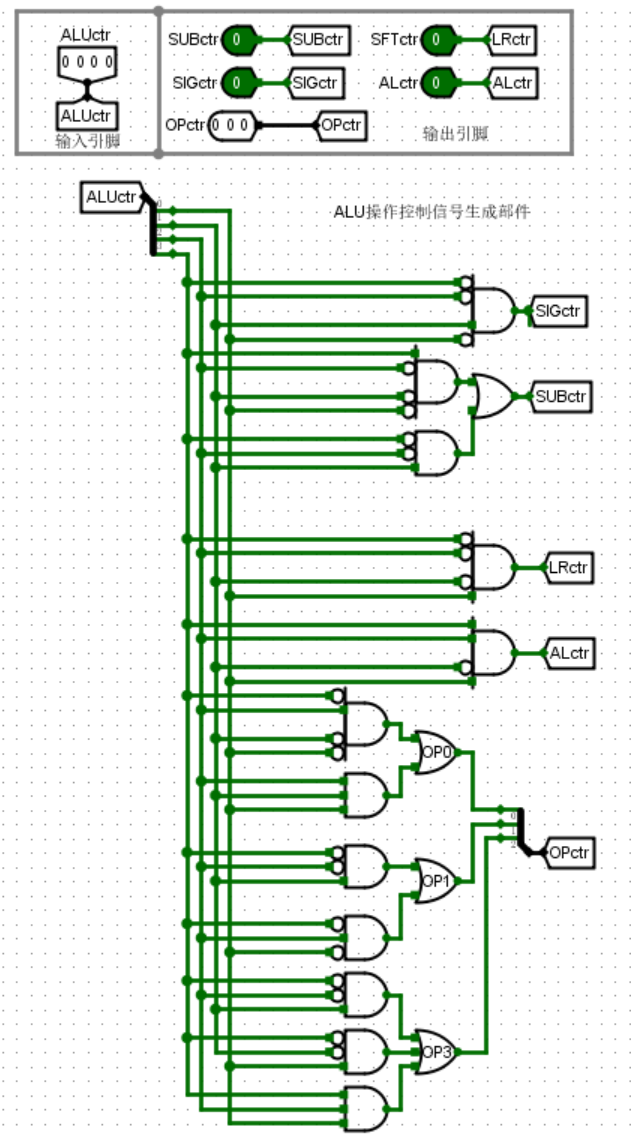
\includegraphics[width=0.8\textwidth]{5.4.2.png}
    \caption{ALU操作控制信号生成部件电路图}
    \end{figure}

    \subsubsection{仿真测试图}
    \begin{figure}[H]
    \centering
    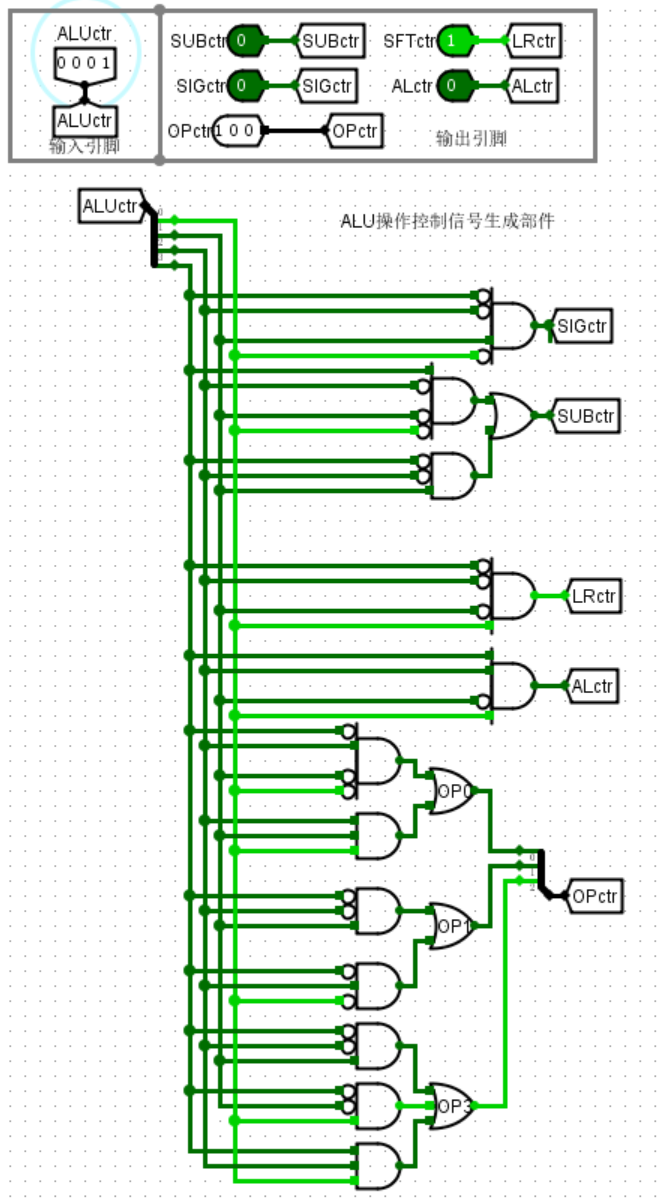
\includegraphics[width=0.4\textwidth]{5.5.1.png}
    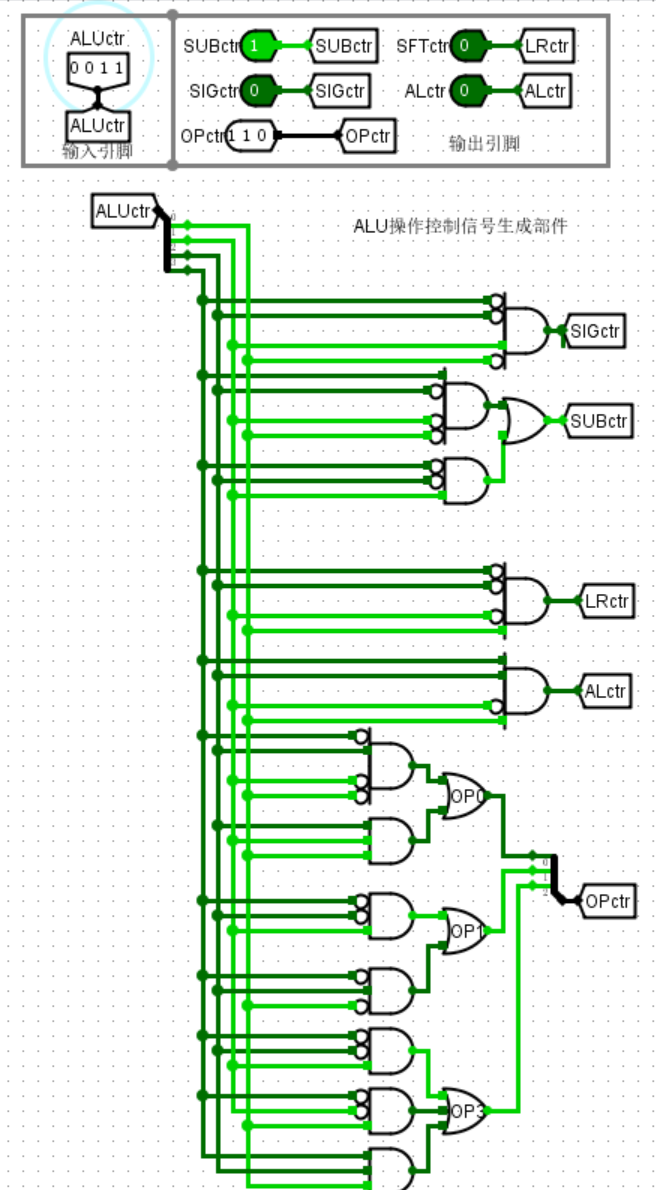
\includegraphics[width=0.4\textwidth]{5.5.2.png}
    \caption{ALU操作控制信号生成部件仿真测试图}
    \end{figure}

    \begin{figure}[H]
    \centering
    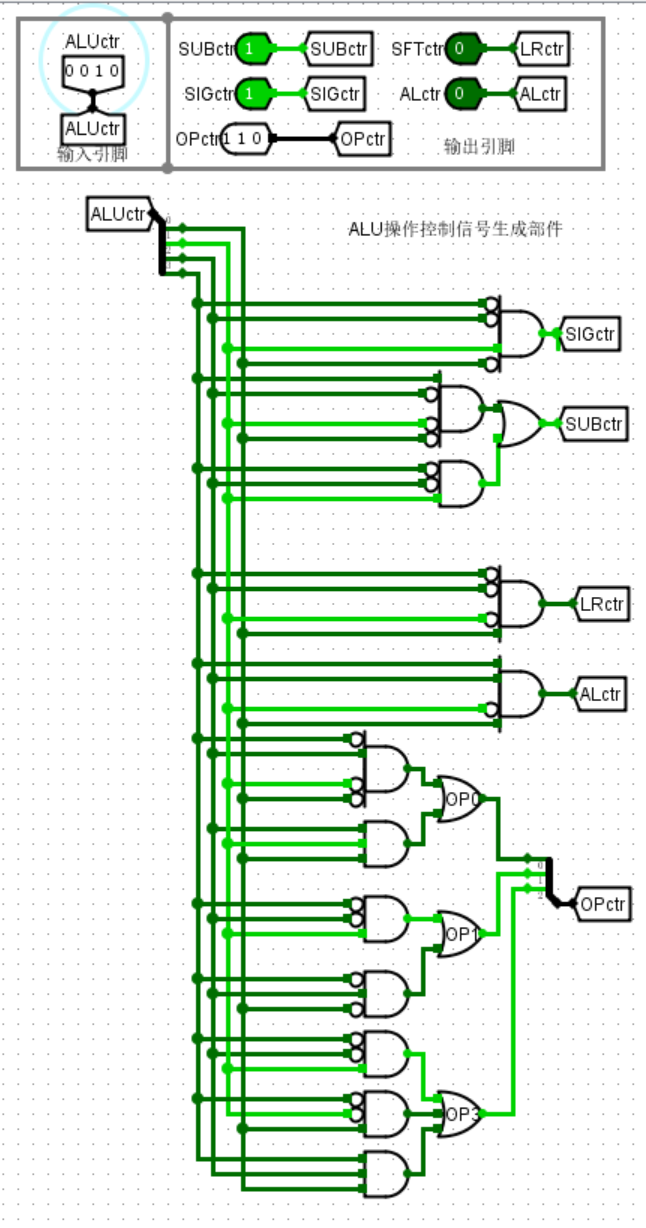
\includegraphics[width=0.4\textwidth]{5.5.3.png}
    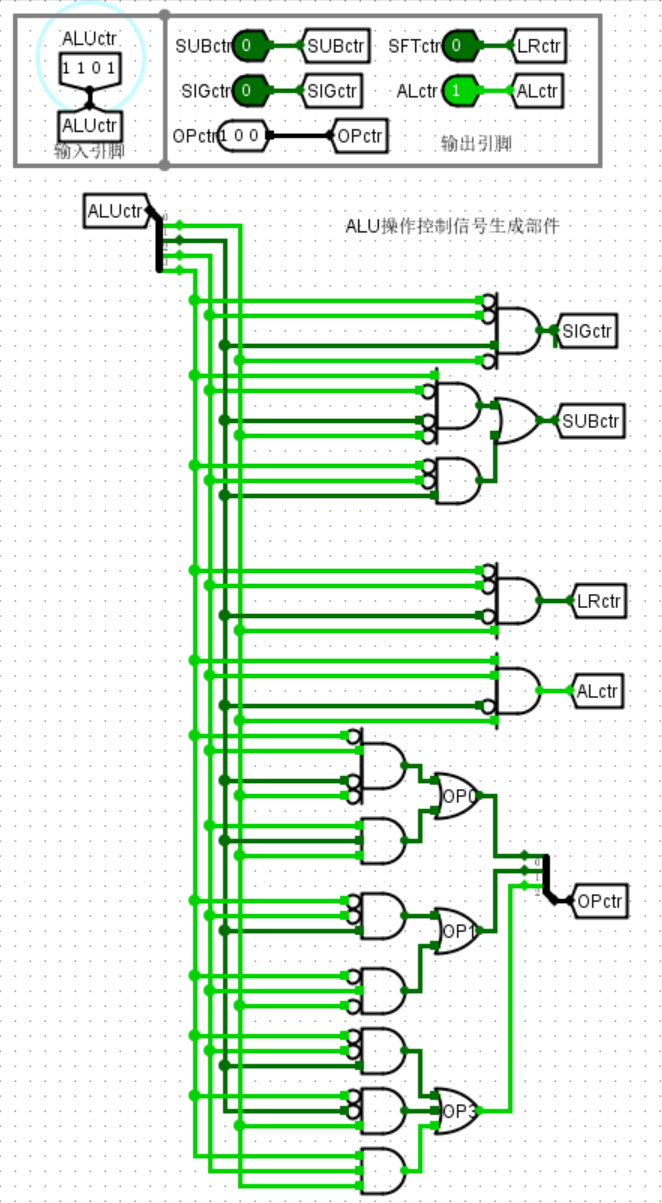
\includegraphics[width=0.4\textwidth]{5.5.4.png}
    \caption{ALU操作控制信号生成部件仿真测试图}
    \end{figure}
    ALUctr=0001, SUBctr=1, SIGctr=0, SFTctr=0, ALctr=0, OPctr=0000;\\
    ALUctr=0011, SUBctr=1, SIGctr=0, SFTctr=0, ALctr=0, OPctr=0000;\\
    ALUctr=0010, SUBctr=1, SIGctr=0, SFTctr=0, ALctr=0, OPctr=0000;\\
    ALUctr=1101, SUBctr=0, SIGctr=0, SFTctr=0, ALctr=0, OPctr=0000;

    \subsubsection{错误现象及分析}
    在完成实验的过程中,没有遇到任何错误。

    \subsection{32位桶形移位器}
    与实验二中 8 位桶形移位器实验相似,只是将其扩展为 32 位,这里用到实验二思考题中的电路。
    \begin{figure}[H]
    \centering
    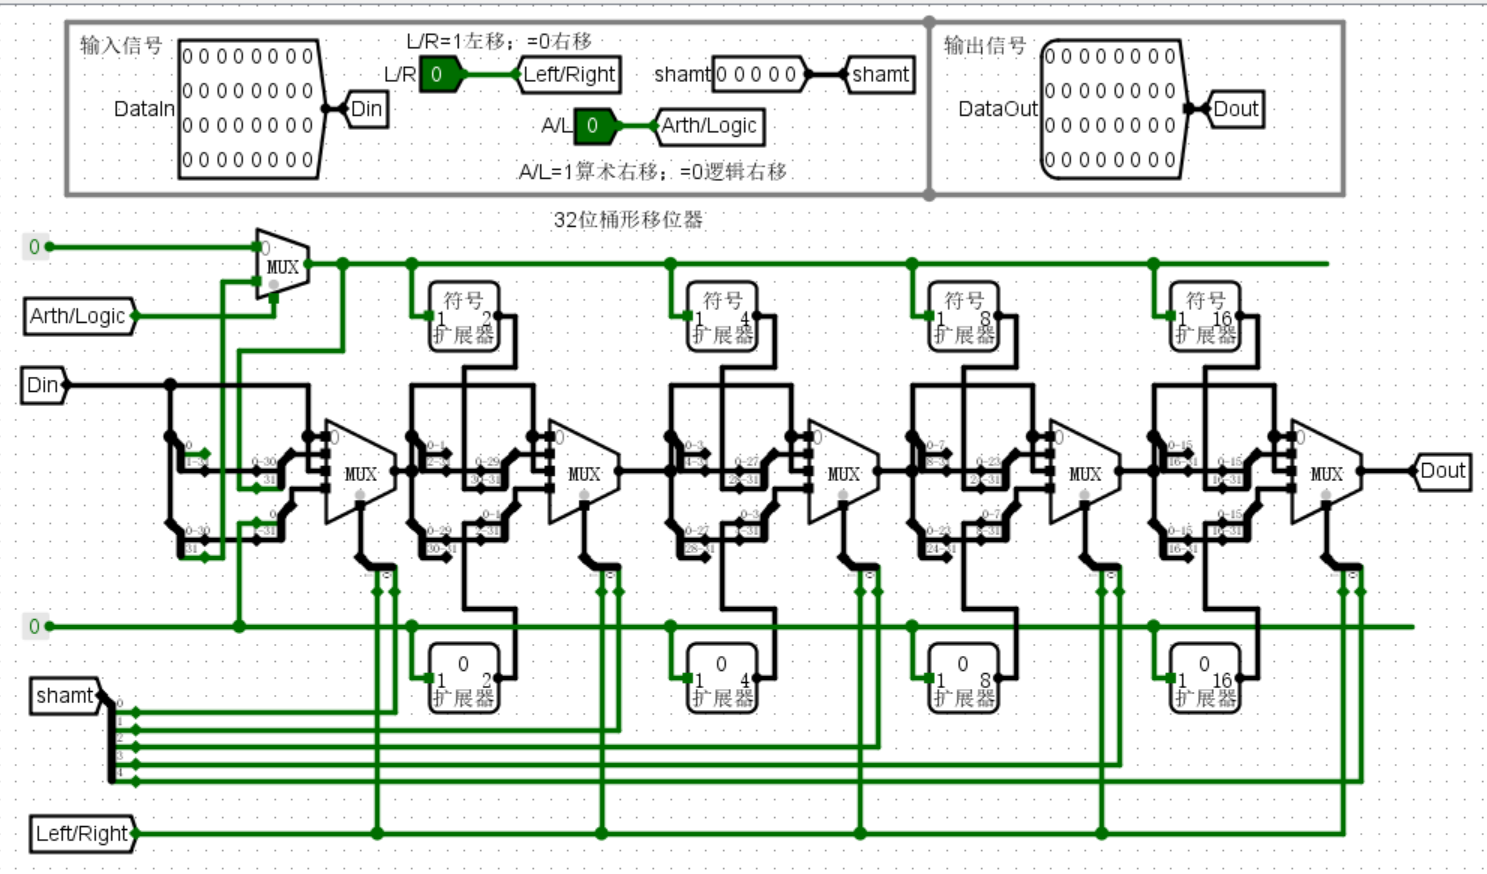
\includegraphics[width=0.4\textwidth]{6.1.png}
    \caption{32位桶形移位器电路图}
    \end{figure}

    \subsection{32 位 ALU}

    \subsubsection{整体方案设计}
    \begin{figure}[H]
    \centering
    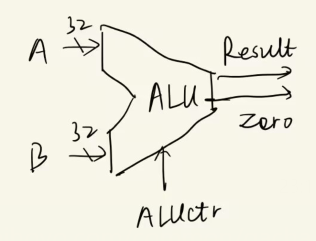
\includegraphics[width=0.4\textwidth]{6.2.png}
    \caption{32位ALU整体方案设计}
    \end{figure}

    \subsubsection{引脚作用}
    \begin{table}[H]
    \centering
    \begin{tabular}{|c|c|}
        \hline
        A[31:0]   & 输入的 A \\ \hline
        B[31:0] & 输入的 B \\ \hline
        ALUctr[3:0]   & 输入的 ALU 控制信号 \\ \hline
        Result[31:0]  & 输出的 C \\ \hline
        Zero  & 输出的是否为 0 的标志位 \\ \hline
    \end{tabular}
    \caption{32位ALU引脚作用}
    \end{table}

    \subsubsection{原理图和电路图}
    \begin{figure}[H]
    \centering
    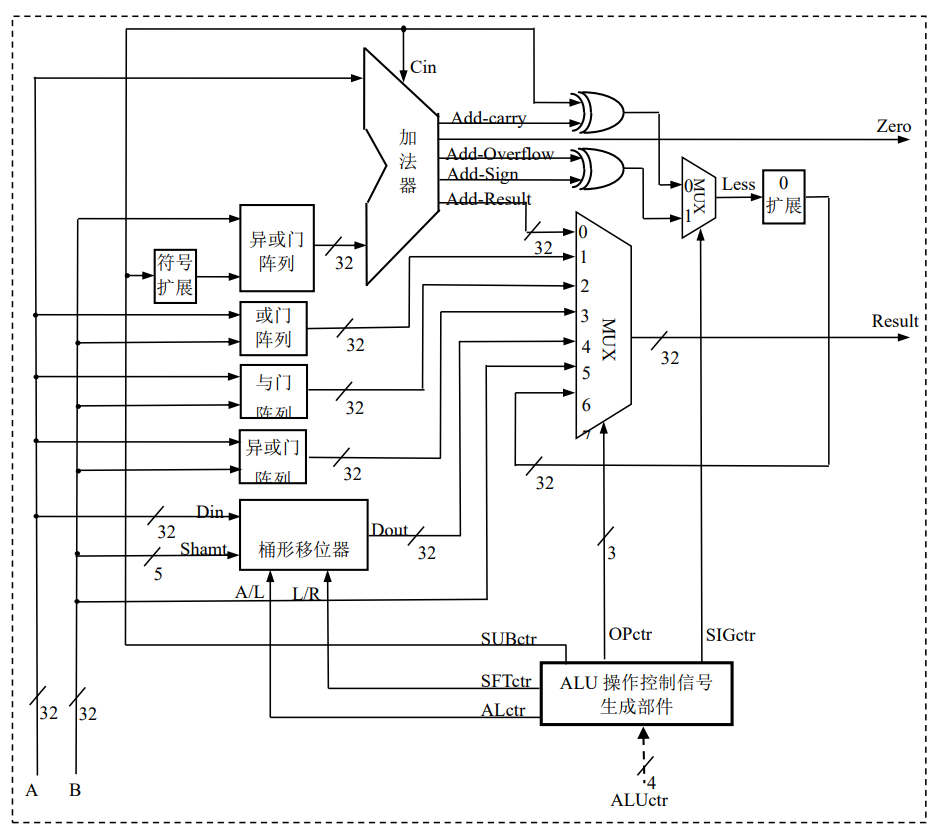
\includegraphics[width=0.8\textwidth]{6.4.1.png}
    \caption{32位ALU原理图}
    \end{figure}

    \begin{figure}[H]
    \centering
    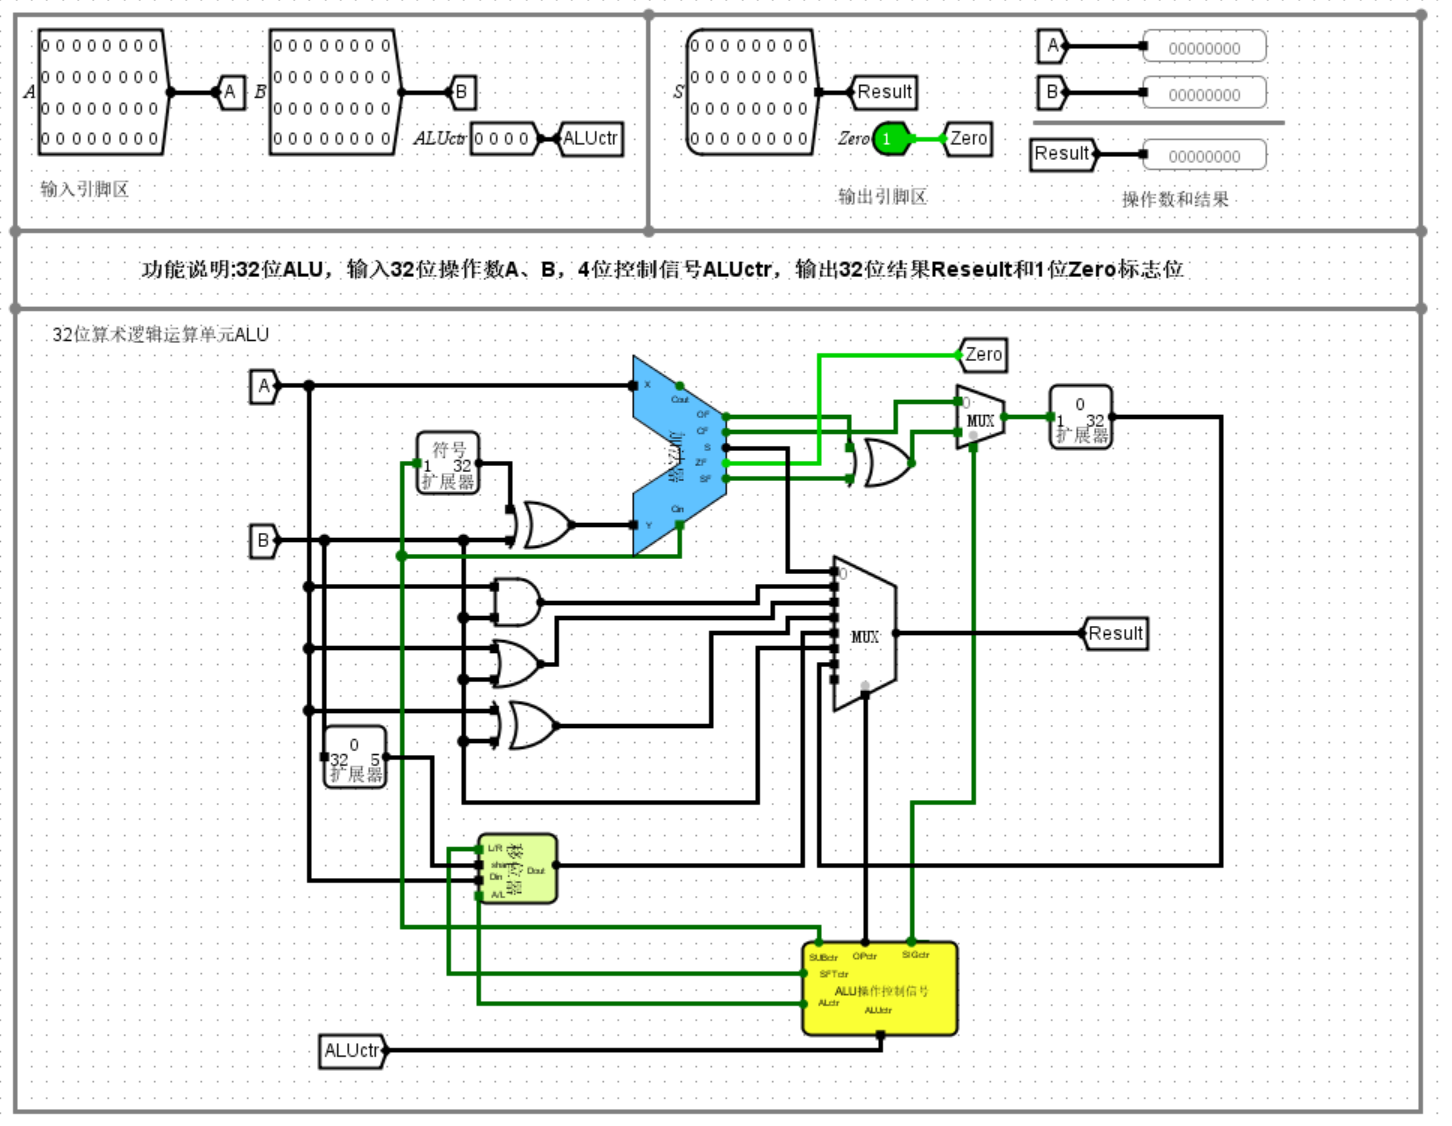
\includegraphics[width=0.8\textwidth]{6.4.2.png}
    \caption{32位ALU电路图}
    \end{figure}

    \subsubsection{仿真测试图}
    \begin{figure}[H]
    \centering
    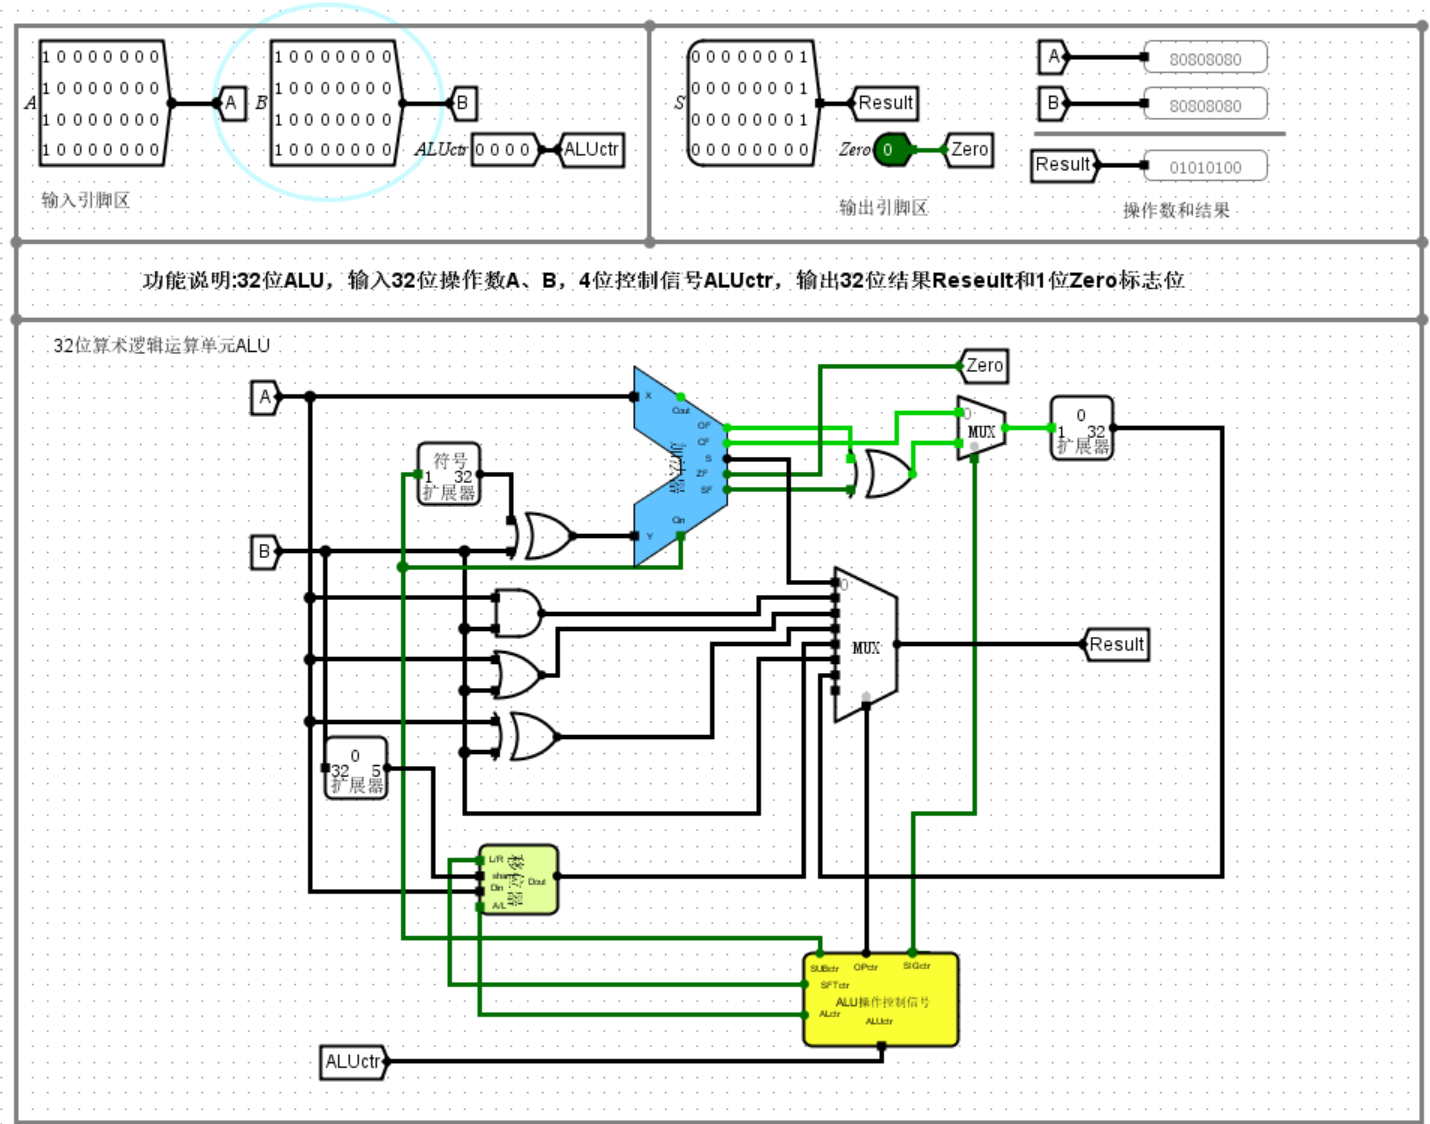
\includegraphics[width=0.4\textwidth]{6.5.1.png}
    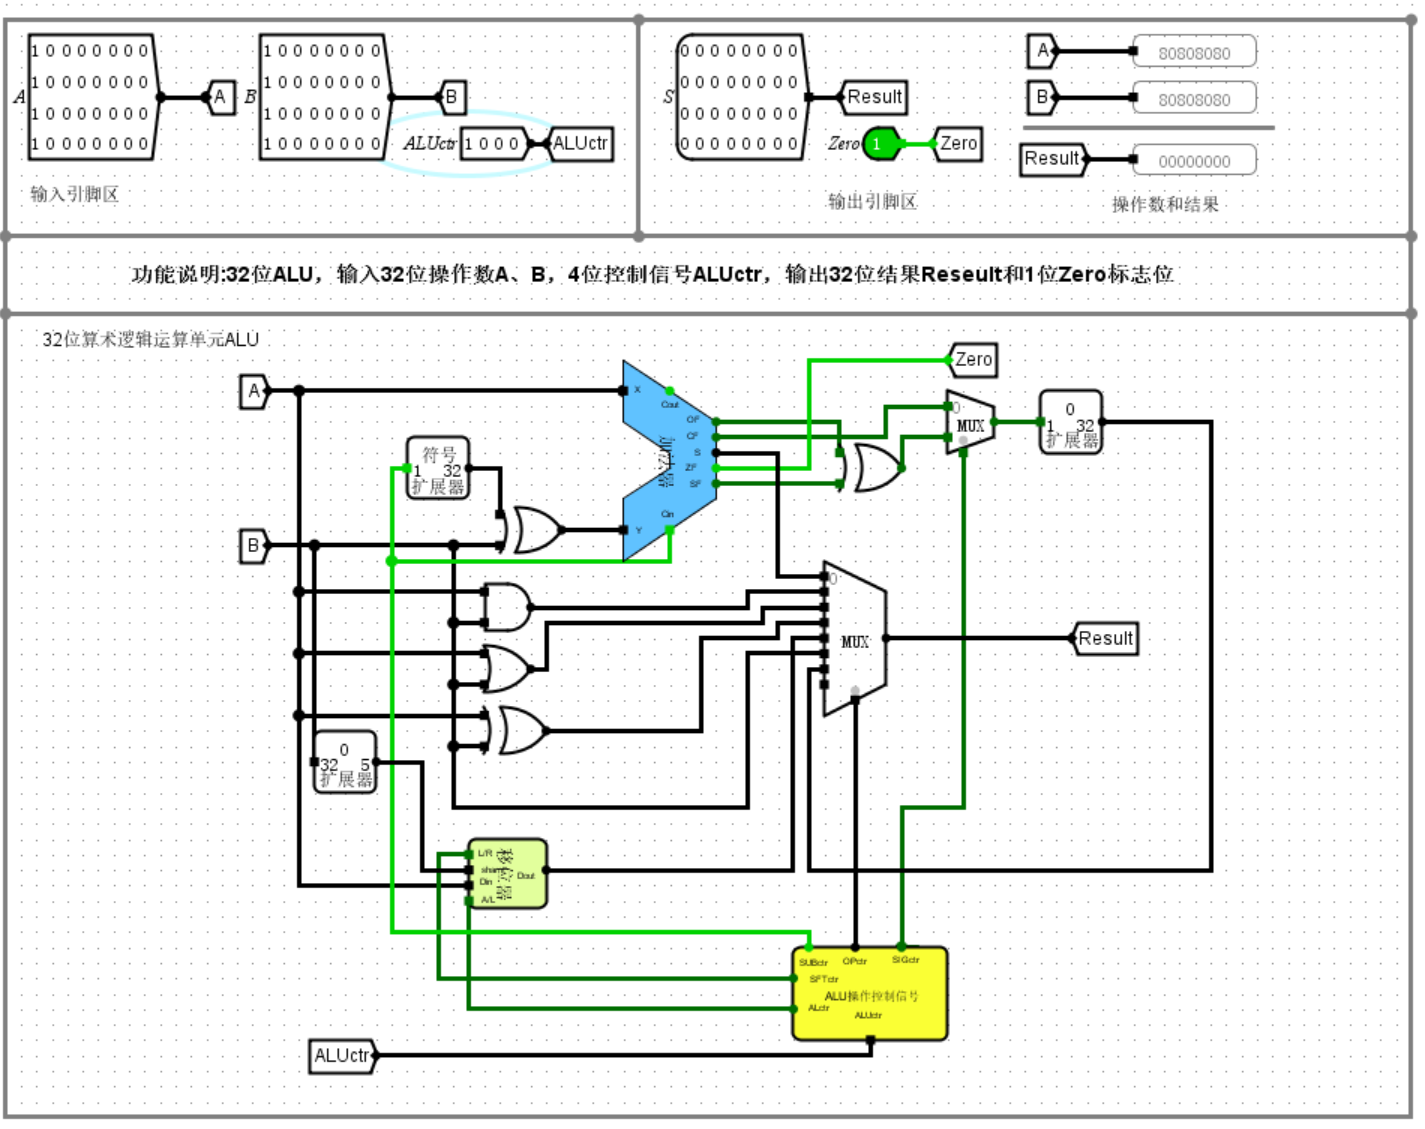
\includegraphics[width=0.4\textwidth]{6.5.2.png}
    \caption{32位ALU仿真测试图}
    \end{figure}

    \begin{figure}[H]
    \centering
    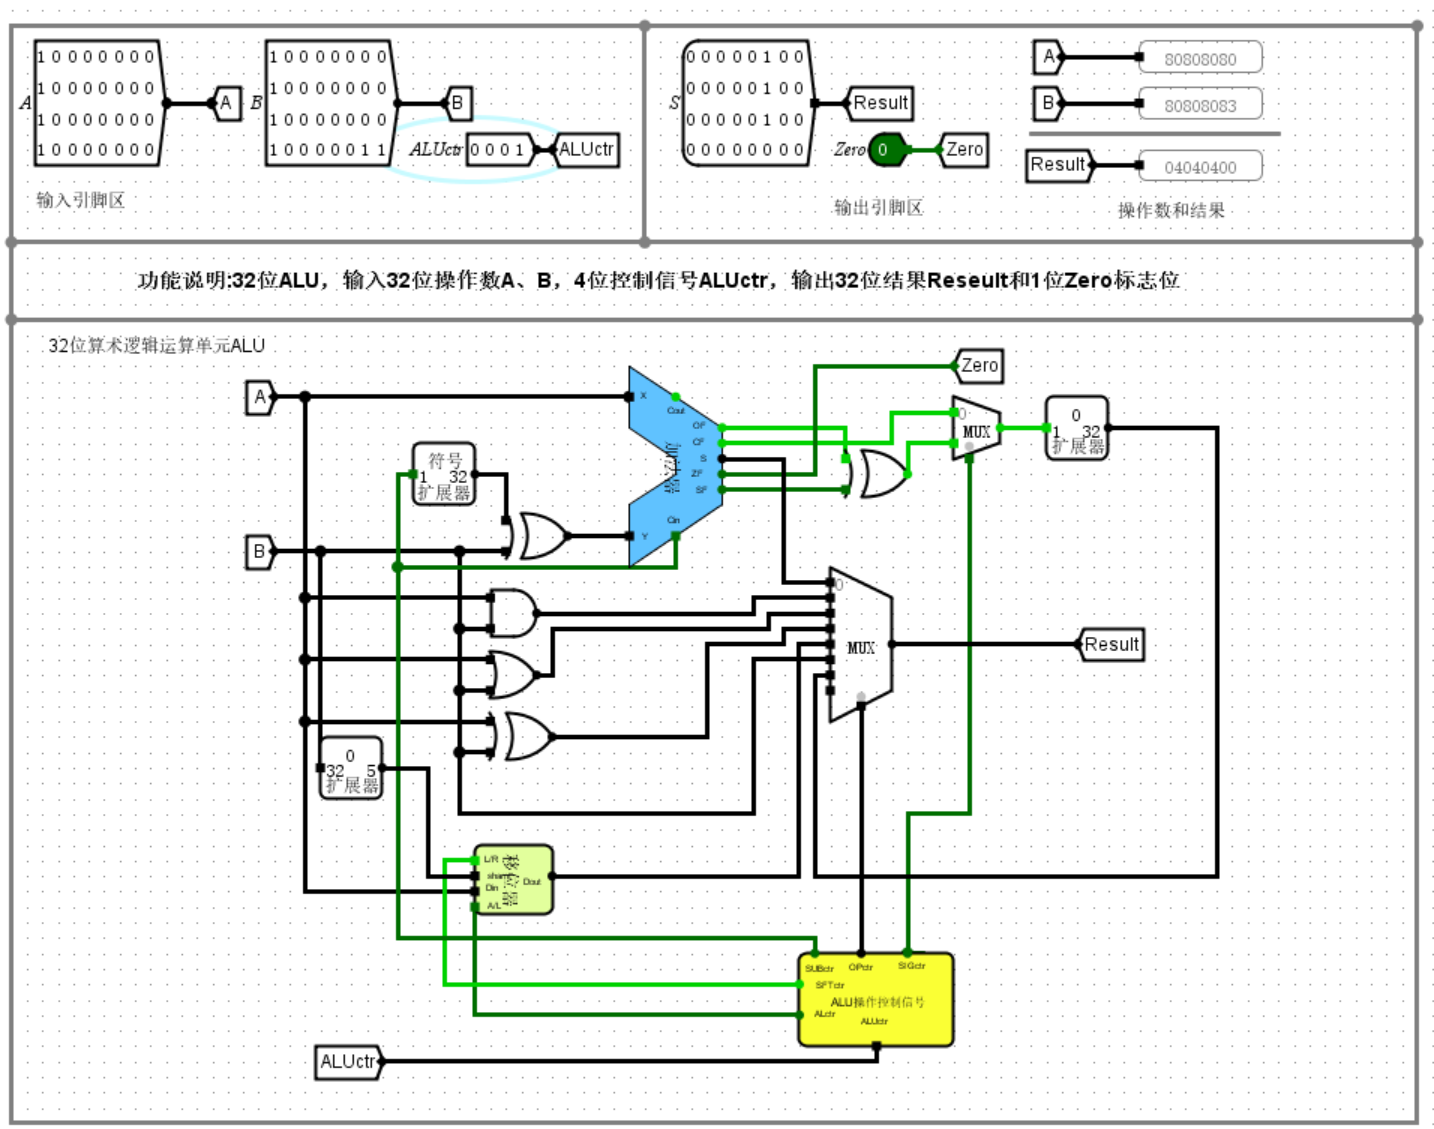
\includegraphics[width=0.4\textwidth]{6.5.3.png}
    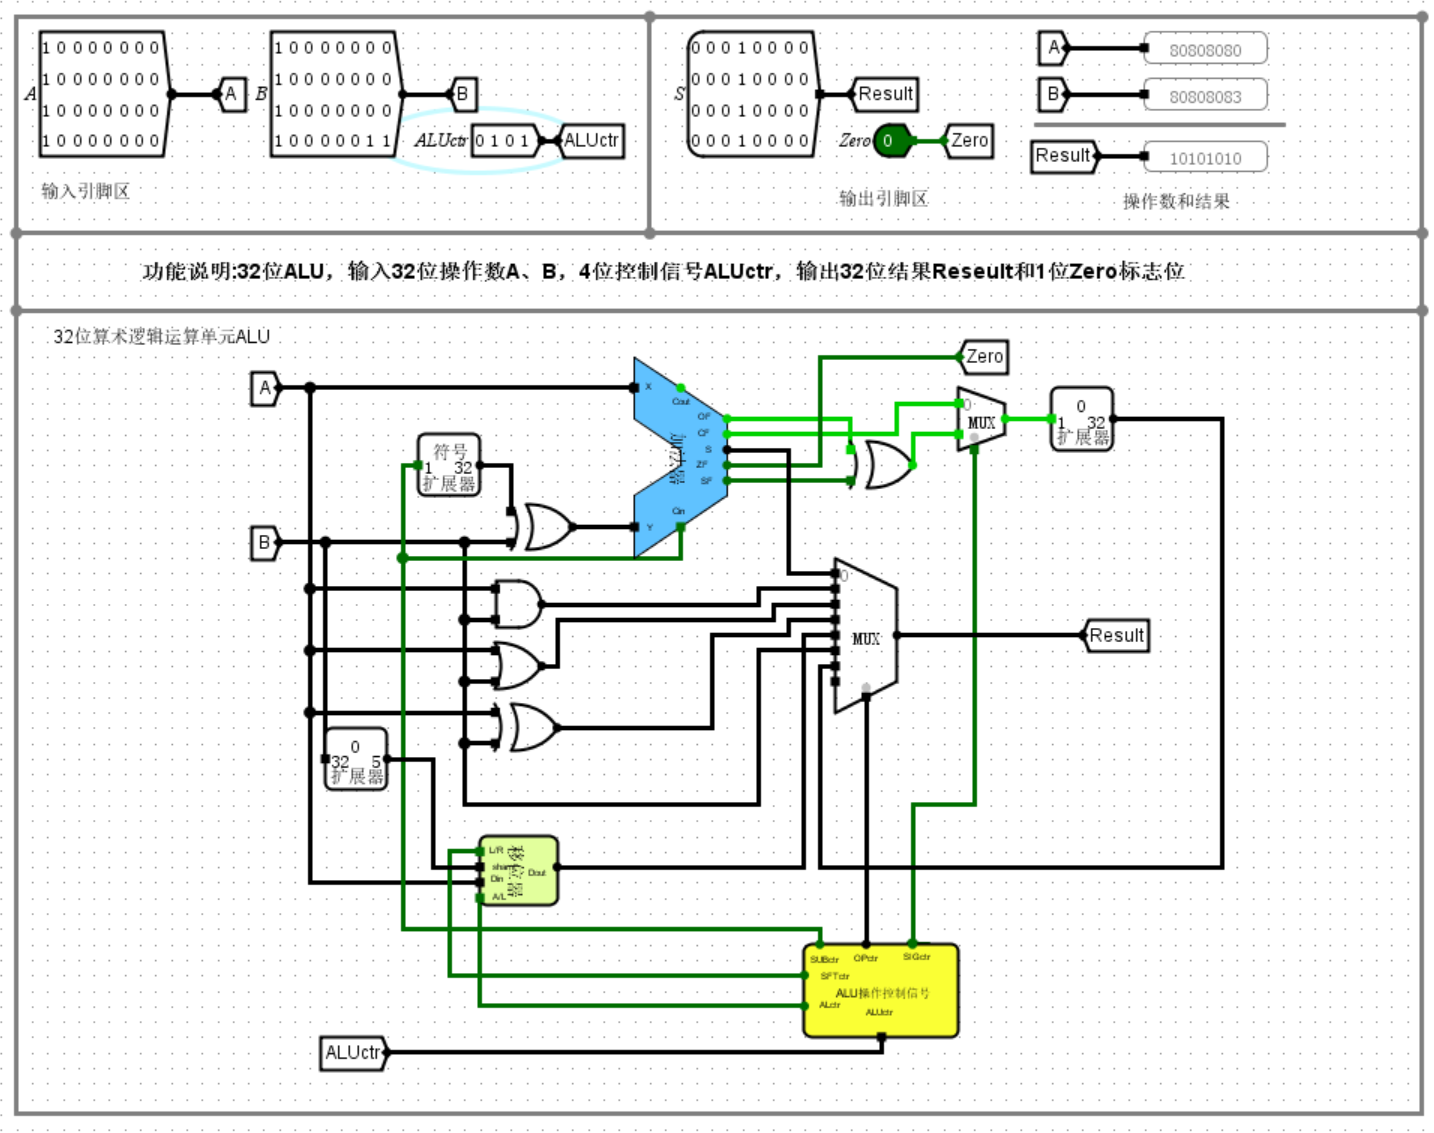
\includegraphics[width=0.4\textwidth]{6.5.4.png}
    \caption{32位ALU仿真测试图}
    \end{figure}
    A=80808080H,B=80808080H,ALUctr=0000,选择加法器的结果输出,Result=01010100H;\\
    A=80808080H,B=80808080H,ALUctr=1000,选择减法器的结果输出,Result=00000000H,Zero=1;\\
    A=80808080H,B=80808083H,ALUctr=0001,选择移位器的结果输出,Result=04040400H;\\
    A=80808080H,B=80808083H,ALUctr=0101,选择移位器的结果输出,逻辑右移Result=80808083H;

    \subsubsection{错误现象及分析}
    在完成实验的过程中,没有遇到任何错误。  


    
    \section{思考题}

    \subsection{利用设计的 ALU,举例说明如何实现一个 32 位整数和一个常量的乘法运算。}
    由于乘法运算是加法和移位的组合,所以可以通过 ALU 的加法器和移位器来实现乘法运算。\\
    可以将 32 位整数和常量的乘法操作分解为若干次移位和加/减法。将常量拆为若干 2 的幂次和/差,使用逻辑左移和加法、减法来实现乘法。

    \subsection{查阅资料,说说除了先行进位加法器以外还有哪些高速并行多位二进制数加法算法,至少简要说明一种算法的实现流程。}
    参考专栏(https://zhuanlan.zhihu.com/p/339963523),进位跳过加法器(Carry-Skip Adder),也叫进位旁路加法器(CBA,carry bypass adder),在CBA单元间,CBA通过旁路让跨位较大的进位跳过了CBA模块内FA的进位链,从而大大减少了较坏情况下的进位延迟。

    \subsection{简要分析加法运算、比较运算和移位运算三种运算中操作数在 ALU 中经过的逻辑门级数。}
    \begin{enumerate}
        \item 加法运算:2 + 3 + 12 + 2 = 19 级逻辑门。

    \begin{enumerate}
        \item 在 ALU 操作控制信号生成部件中,从 ALUctr 到 SUBctr,计 2 级逻辑门。
        \\
        \item 在符号扩展进入异或门时,计 3 级逻辑门。
        \item 在加法器内:
        \begin{enumerate}
        \item 在 4-bit CLA 中,从得到 X, Y 到生成所有进位、组间进位生成函数/进位传递函数,计 3 级逻辑门;到生成所有和数,计 6 级逻辑门。从得到 Cin 到生成所有进位,计 2级逻辑门;到生成所有和数,计 5 计逻辑门。
        \item 在 16-bit CLA 中,从得到 X, Y 到生成所有进位,计 5 级逻辑门;到生成所有和数,计 10 级逻辑门。从得到 C0 到生成所有进位,计 2 级逻辑门;到生成所有和数,计7 级逻辑门。
        \item 在 32-bit 加法器中,从得到 X, Y 到生成和数,计 12 级逻辑门。
        \end{enumerate}
        
        \item 在离开加法器后,经过由 OPctr 控制的 MUX,计 2 级逻辑门。

    \end{enumerate}
    \item 比较运算:即减法运算,与加法相同,关键路径为 19 级逻辑门。
    \item 移位运算:关键路径为从 ALUctr 生成 ALctr 后,再在移位器内经过 5 次 MUX 得到结果后,再通过 OPctr 控制的 MUX 得到 Result.共需要 $1 + 5 × 2 + 2 = 13$ 级逻辑门。


    \end{enumerate}
\end{document}